\documentclass[11pt, oneside]{article}
\usepackage[margin=1in]{geometry}
\geometry{letterpaper}
\usepackage{booktabs}
\usepackage{hyperref}
\usepackage{enumitem}
\usepackage{float}
\usepackage{caption}
\usepackage{subcaption}
\usepackage[numbers]{natbib}
\usepackage{graphicx}
\usepackage{amssymb}
\usepackage{amsmath}
\usepackage{array}
\usepackage{longtable}
\usepackage{xcolor}
\usepackage{tabularx}
\usepackage{setspace}
\usepackage{adjustbox}
\usepackage{tikz}
\usetikzlibrary{positioning,arrows.meta}

\hypersetup{
    colorlinks=true,
    linkcolor=blue,
    citecolor=blue,
    urlcolor=blue
}
\graphicspath{{figures/}{../figures/}}
\captionsetup{font=small}
\setlength{\textfloatsep}{8pt}
\setlength{\floatsep}{6pt}
\setlength{\intextsep}{6pt}
\renewcommand{\topfraction}{0.9}
\renewcommand{\bottomfraction}{0.8}
\renewcommand{\textfraction}{0.07}
\renewcommand{\floatpagefraction}{0.85}
\setcounter{topnumber}{3}
\setcounter{bottomnumber}{2}
\setcounter{totalnumber}{5}

\newcommand{\run}[1]{\texttt{#1}}
\newcommand{\best}[1]{\textbf{#1}}

% ============================================================
% TITLE BLOCK --- kept as required by the template
% ============================================================
\title{CS781 Capstone Project:\\
In-House Legal Intelligence System}
\author{
    Sanskaar Srivastava \\
    220967 \\
    {\tt sanskaars22@iitk.ac.in}\\
    Indian Institute of Technology Kanpur (IIT Kanpur)
}
\date{}

\begin{document}
\maketitle

\begin{abstract}
A law firm that cannot send client documents to outside services needs legal language technology it can train and
host itself. I built such a stack under the capstone's constraints: every model is trained from scratch on the
official Indian legal corpus, with 50--300M parameters and free Kaggle GPUs. In Phase~1 I pretrained five language models (58--101M parameters) on Supreme Court
judgments; the best, a 101M-parameter decoder with RMSNorm, SwiGLU, rotary positions and grouped-query attention,
reached a BERTScore of 0.8407 on passage continuation with minimum Bayes risk (MBR) decoding. Four $\approx$100M models were then adapted to six tasks:
named entity recognition, rhetorical roles, judgment prediction, statute identification, summarization and prior
case retrieval. I compared full and partial fine-tuning, LoRA, rsLoRA, LoRMA, IA$^3$, BitFit, Houlsby adapters and
distillation, together with CRF layers, long-document reading strategies and decoding computed from training data.
Across the reading tasks, M5's bidirectional prefix-LM pretraining was a strong starting point, while task structure
often mattered as much as the backbone: CRF decoding, thresholds and retrieval normalisation produced large gains.
The results also have clear limits: scarce data, long documents, rare labels and metrics that do not establish
factual correctness.
\end{abstract}

% ============================================================
\section{Competition Result}
% ============================================================
\noindent
\textbf{Codabench username:} s\_220967
\hfill
\textbf{Roll number:} 220967

\medskip
\noindent
Table~\ref{tab:leaderboard} lists the best valid score of each phase. The template lists six phases; Phase~7 (prior
case retrieval) was added to the competition later and is reported in the same way.

\begin{table}[H]
\centering
\caption{Best phase results.}
\label{tab:leaderboard}
\begin{tabular}{clccc}
\toprule
Phase & Task & Primary metric (value) & Rank & Valid submissions \\
\midrule
1 & Legal LM Pretraining & BERTScore F1 0.8407 & 14 / 142 & 11 \\
2 & Legal NER & strict macro-F1 0.5122 & 76 / 133 & 27 \\
3 & Rhetorical role prediction & macro-F1 0.5713 & 19 / 131 & 41 \\
4 & Court judgment prediction & macro-F1 0.7609 & 38 & 18 \\
5 & Legal statute identification & macro-F1 0.3664 & 80 / 133 & 7 \\
6 & Abstractive summarization & BERTScore F1 0.8381 & 68 / 129$^\dagger$ & 6 \\
7 & Prior case retrieval & Micro-F1@7 0.4318 & 49 & 8 \\
\bottomrule
\end{tabular}
\end{table}

\noindent
\textbf{Total valid Codabench submissions across all phases:} 118
\quad
\textbf{Date ranks were recorded:} 9 November 2026

\noindent{\footnotesize Rank = position of my best submission on the phase leaderboard / leaderboard entries (the entry
count for Phases~4 and~7 could not be retrieved). Valid = submissions that finished scoring; the course minimum is 4 in
Phase~1 and 6 in Phases~2--7. $^\dagger$Phase~6 was still open when the rank was recorded.}

% ============================================================
\section{Introduction and Problem Description}
% ============================================================
The capstone asked me to build a small legal language model from scratch, then adapt it to six Indian legal tasks
from the IL-TUR benchmark~\cite{iltur}. The tasks cover passage continuation, named-entity recognition, rhetorical
role classification, judgment prediction, statute identification, summarisation and prior-case retrieval. They use
different metrics, including exact span F1, macro-F1, BERTScore and Micro-F1@7.

Models had to use 50--300M parameters and only the official data; my downstream systems had to start from my Phase~1
checkpoints. Training was limited to two Kaggle T4 GPUs in 12-hour sessions, so I compared four architectures and
several adaptation methods, including the required LoRMA~\cite{lorma} and knowledge distillation. I did not use
external data, search hyperparameters or run multiple seeds. Table~\ref{tab:links} connects the main data findings
to the decisions they informed; later sections report the experiments and their limitations.

% ============================================================
\section{Data Analysis and Preprocessing}
% ============================================================
\subsection{Sources and official splits}
I used only the official \texttt{Exploration-Lab/CS-781-Capstone} data. Table~\ref{tab:data} lists the splits.
For local evaluation, I held out 10 of the 70 Phase~2 training documents and 200 Phase~6 training pairs; Phase~6
has no official development split. The Phase~3 files are split by domain, and Phase~7 provides queries, relevant
cases and candidate pools.

\begin{table}[htbp]
\centering\small
\caption{Official splits (q = queries, c = candidate pool); median length in words (Phase~3: per sentence; Phase~6:
document $\to$ summary). $^\dagger$After removing the test cases contained in \texttt{dev.json}.}
\label{tab:data}
\begin{adjustbox}{max width=\textwidth}\begin{tabular}{llllll}
\toprule
Phase & Train & Dev & Test & Median length & Metric\\
\midrule
1 LM & 1.3\,GB SC text (of 19.2\,GB) & --- & 1{,}000 prompts & 512 / 128 words & BERTScore F1\\
2 NER & 70 docs, 8{,}393 spans & 10 docs (held out) & 35 docs & 4{,}498 words & strict macro-F1\\
3 RR & 80 docs, 16{,}845 sent. & 10 docs, 2{,}142 sent. & 10 docs, 2{,}197 sent. & 27 words/sent. & macro-F1\\
4 CJPE & 31{,}677 cases & 994 cases$^\dagger$ & 1{,}517 cases & 2{,}030 words & macro-F1\\
5 LSI & 42{,}750 docs & 10{,}181 docs & 13{,}019 docs & 430 words & macro-F1 (100)\\
6 Summ. & 7{,}030 pairs & 200 held out & 100 docs & 3{,}146 $\to$ 641 & BERTScore F1\\
7 PCR & 827 q / 4{,}320 c & 118 q / 1{,}023 c & 237 q / 1{,}727 c & 3{,}947 words & Micro-F1@7\\
\bottomrule
\end{tabular}
\end{adjustbox}
\end{table}

\subsection{Findings that shaped the design}\label{sec:links}
Figure~\ref{fig:data} and Table~\ref{tab:links} summarise the data patterns that influenced my choices. I made
these choices using training and validation data, not Codabench scores.
\begin{itemize}[nosep]
\item The pretraining files cover the Supreme Court (1.3\,GB), High Courts (10.7\,GB), Tribunals (6.5\,GB) and Acts (0.7\,GB).
\item Phase~2 requires exact character offsets: a token span such as \emph{``Ghosh,''} must be trimmed to \emph{``Ghosh''}.
\item Phase~4 has 31{,}677 distinct training texts in 37{,}387 rows.
\item In Phase~7, \emph{CITATOR INFO} matched the query in 105 of 214 sampled relevant pairs, so I removed it.
\end{itemize}

\begin{figure}[htbp]
\centering
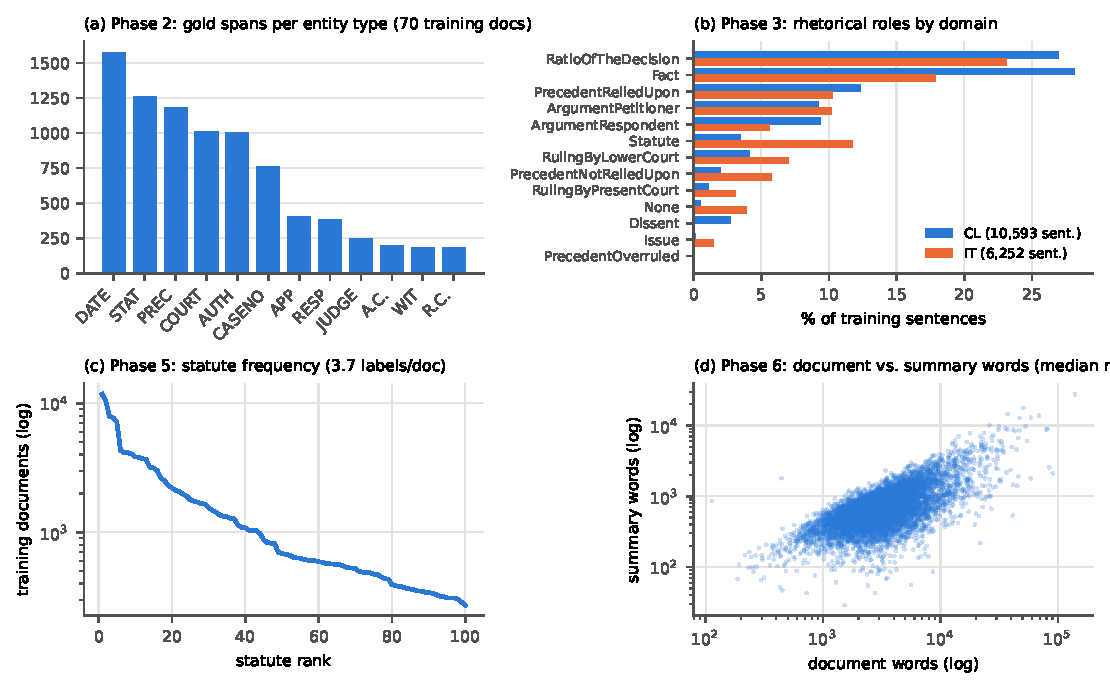
\includegraphics[width=0.62\textwidth]{data_panels.pdf}
\caption{Training-data statistics that shaped the design (computed from the official files).}
\label{fig:data}
\end{figure}

\subsection{Preprocessing decisions}\label{sec:prep}
I used one byte-level BPE tokenizer~\cite{bpe} (50{,}001 tokens, no case or text normalisation) across phases.
For Phase~2, I added character offsets without changing token IDs, then converted BIO tag runs back to spans and
trimmed boundary punctuation, brackets and possessives. This raises the round-trip strict macro-F1 ceiling from
0.605 to 0.979 (Table~\ref{tab:ceiling}). I kept the supplied Phase~3 sentences, cutting the roughly 1\% longer
than 256 tokens. Phase~4's \texttt{dev.json} included all 1{,}517 labelled test cases; I removed them, used the
remaining 994 cases for validation and deduplicated training data without using test labels. I merged duplicate
Phase~5 records by taking the union of their labels. In Phase~7, I removed \emph{CITATOR INFO} and extracted each
case date from its header or, if absent, from the latest year mentioned.

\begin{table}[htbp]
\centering\scriptsize
\caption{Data findings and the design decisions they caused.}
\label{tab:links}
\begin{adjustbox}{max width=\textwidth}
\begin{tabular}{c>{\raggedright\arraybackslash}p{8.4cm}>{\raggedright\arraybackslash}p{6.2cm}c}
\toprule
Ph. & Finding (training data) & Decision & Sec.\\
\midrule
1 & Test prompts closest to Supreme Court text (fertility 1.070 vs.\ 1.085 for a uniform mix) & Tokenizer and pretraining on that file only & \ref{sec:p1}\\
1 & $\approx$200M tokens per model fit the budget ($\approx$2 per parameter) & Fixed shape; effort spent on throughput & \ref{app:arch}\\
2 & 40\% of gold spans do not end on a word boundary & Character offsets, trimming rules (ceiling 0.979) & \ref{sec:prep}\\
2 & One wrong tag breaks an exact span; softmax can emit invalid BIO runs & CRF output layer & \ref{sec:p2}\\
2 & Parties in the first 256 tokens (98\%/94\%); half of all mentions beyond token 1{,}024 & Overlapping windows, 256-token preamble & \ref{sec:p2}\\
2 & Names repeat within a judgment & Vote and propagate rules & \ref{sec:p2}\\
3 & Roles follow the order of a judgment and differ between CL and IT & Document windows, sentence CRF, training Viterbi & \ref{sec:p3}\\
3 & Two roles absent from development (macro-F1 bound 11/13) & Ensembles rather than single-run selection & \ref{sec:p3}\\
4 & Median case 2{,}030 words; the outcome is stated at the end & Chunk reader, tail reading, section analysis & \ref{sec:p4}\\
4 & Labelled test cases inside \texttt{dev.json}; 41\% positive in training vs.\ 50\% in dev & Removed (994 dev cases); decision threshold & \ref{sec:prep}\\
5 & 3.7 of 100 statutes per document; 272--11{,}731 documents per statute & Log-odds biases, per-statute thresholds & \ref{sec:p5}\\
5 & 78\% of documents fit in $4\times512$ tokens & Read the head $4\times512$ tokens & \ref{sec:p5}\\
6 & Compression 4.6; 79\% of summary bigrams occur in the document; no dev split & Conditional LM on head+tail; 200 held out & \ref{sec:p6}\\
7 & A query is never its own answer; relevant cases are earlier & Self and date rules & \ref{sec:p7}\\
7 & A candidate is relevant to $\approx$1 query; CITATOR INFO leaks labels & Column normalisation; field deleted & \ref{sec:p7}\\
7 & Other queries as answers: 19.4\% in training vs.\ 2.0\% in dev & Query penalty, also every setting with $p{=}0$ & \ref{sec:p7}\\
\bottomrule
\end{tabular}
\end{adjustbox}
\end{table}

% ============================================================
\section{Approach and Model Evolution}\label{sec:approach}
% ============================================================
\subsection{Phase-1 foundation model}\label{sec:p1}
I trained five models in sequence (Table~\ref{tab:arch}). Model~1, a GPT-2-style decoder~\cite{radford2019gpt2},
produced loops (\emph{``to the High Court to the High Court''}). Model~2 added rotary positions~\cite{rope} and
grouped-query attention~\cite{gqa} (12 query heads sharing 4 key/value heads) at 101M parameters; it was stopped at 74\%
of its epoch. Model~3, a GRU encoder--decoder with Bahdanau attention~\cite{bahdanau}, fitted only 98M tokens because of
its sequential recurrence. Model~4 keeps Model~2's shape but uses RMSNorm~\cite{rmsnorm}, SwiGLU~\cite{swiglu}, no
biases, scaled residual initialisation, a tied output layer, 65k-token batches and a chunked cross-entropy that never
builds the full logit tensor; it completed 214M tokens (Fig.~\ref{fig:arch}). Model~5 is that network trained as a
prefix-LM~\cite{t5} (a 64--640-token prompt read bidirectionally, loss on the continuation only). Parameter counts were
verified by summing all parameter tensors.

The sequence tests several design choices under the same compute limit: M1 was the starter baseline; M2 added RoPE
and grouped-query attention; M3 tested a recurrent encoder--decoder; M4 kept M2's shape but used a faster modern
training recipe; and M5 changed M4 to prefix-LM training. M4 processed the most data, while M3's recurrence limited
it to 98M tokens. I carried M2--M5 into downstream tasks; M1 served only as a baseline. Appendix~\ref{app:arch}
records the architecture trade-offs in more detail.

\begin{table}[htbp]
\centering\small
\caption{Phase 1 models (validation loss in nats/token, $^*$continuation tokens only; LB = Codabench BERTScore with each
model's original decoding). M2--M5 are adapted in Phases 2--7.}
\label{tab:arch}
\begin{adjustbox}{max width=\textwidth}
\begin{tabular}{@{}lllllrrr@{}}
\toprule
Model & Type & Shape & Position & Norm, MLP & Params & Val.\ loss & LB\\
\midrule
M1 & decoder (GPT-2 style) & 8L, $d$=560, 8 heads, ctx 2048 & sinusoidal & LayerNorm, GELU & 58.2M & 4.742 & 0.7830\\
M2 & decoder & 10L, $d$=768, GQA 12/4, ctx 1024 & RoPE & LayerNorm, GELU & 101.4M & 3.007 & 0.8087\\
M3 & GRU enc.--dec. & 2L bi-GRU + 2L GRU, $h$=1024 & recurrent & --- & 91.7M & 4.808$^*$ & 0.7874\\
M4 & modern decoder & 10L, $d$=768, GQA 12/4, ctx 1024 & RoPE & RMSNorm, SwiGLU & 101.3M & \best{2.992} & \best{0.8324}\\
M5 & prefix-LM & as M4 & RoPE & RMSNorm, SwiGLU & 101.3M & --- & 0.8300\\
\bottomrule
\end{tabular}
\end{adjustbox}
\end{table}

\begin{figure}[htbp]
\centering
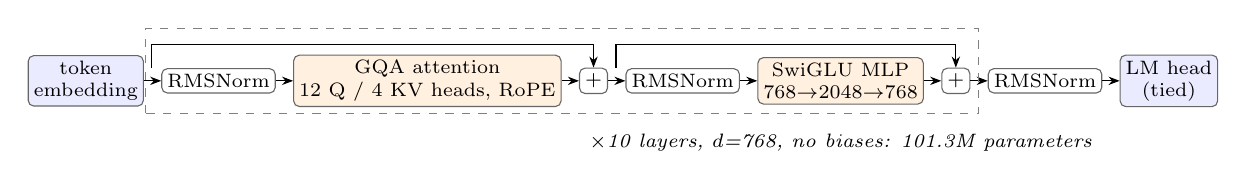
\begin{tikzpicture}[font=\scriptsize, >={Stealth[length=4pt]}, node distance=2.2mm,
  b/.style={draw=black!60, rounded corners=2pt, align=center, inner sep=2pt, fill=#1}, b/.default=white]
\node[b=blue!8] (e) {token\\embedding};
\node[b, right=of e] (n1) {RMSNorm};
\node[b=orange!12, right=of n1] (at) {GQA attention\\12 Q / 4 KV heads, RoPE};
\node[b, right=of at] (p1) {$+$};
\node[b, right=of p1] (n2) {RMSNorm};
\node[b=orange!12, right=of n2] (ff) {SwiGLU MLP\\768$\to$2048$\to$768};
\node[b, right=of ff] (p2) {$+$};
\node[b, right=of p2] (n3) {RMSNorm};
\node[b=blue!8, right=of n3] (o) {LM head\\(tied)};
\foreach \a/\b in {e/n1,n1/at,at/p1,p1/n2,n2/ff,ff/p2,p2/n3,n3/o} \draw[->] (\a) -- (\b);
\draw[->] ([xshift=-1.2mm]n1.north west) -- ++(0,.3) -| (p1.north);
\draw[->] ([xshift=-1.2mm]n2.north west) -- ++(0,.3) -| (p2.north);
\draw[dashed, black!50] ([xshift=-2mm,yshift=-2.5mm]n1.south west) rectangle ([xshift=1mm,yshift=5mm]p2.north east);
\node[anchor=north, font=\scriptsize\itshape] at ([yshift=-2.5mm]ff.south) {$\times$10 layers, $d$=768, no biases: 101.3M parameters};
\end{tikzpicture}
\caption{The Model~4 decoder (Model~5: the same network with a bidirectional prompt mask).}
\label{fig:arch}
\end{figure}

\textbf{Decoding.} With a pseudo-validation set cut from the test prompts (words 1--384 as prompt, 385--512 as
reference) and a key/value-cache re-implementation of Model~4, I compared 28 settings: greedy, $n$-gram blocking,
repetition~\cite{ctrl} and frequency penalties, top-$p$~\cite{nucleus} and min-$p$ sampling, beam and contrastive
search~\cite{contrastive}, and MBR selection~\cite{mbr}; pseudo-validation tracked Codabench within 0.002
(Appendix~\ref{app:p1}). The best single setting decodes greedily with a 4-gram block and repetition penalty 1.2 and
keeps the first 128 words (0.8363, from 0.8324). The best submission generates 14 candidates per prompt (six
greedy/beam variants, eight seeded top-$p$/min-$p$ samples) and returns the one with the highest mean BERTScore against
the others (MBR, 0.8407).

\subsection{Transfer protocol (Phases 2--7)}
Each downstream model starts from M2--M5 with the tokenizer unchanged and a task-specific output layer
(Fig.~\ref{fig:overview}). For tagging, classification and retrieval, I removed the decoders' causal mask so each
prediction could use both left and right context. M5 had already seen bidirectional prompts during pretraining;
M3 used its bidirectional GRU encoder. I implemented the adaptation methods myself, including full and partial
fine-tuning, LoRA, rsLoRA, LoRMA, IA$^3$, BitFit, Houlsby adapters and distillation. Table~\ref{tab:techs} shows
which methods I tested; Appendix~\ref{app:techs} gives their details.

No backbone won every task. M5 led Phases~2--4 and was the strongest learned Phase~7 retriever; M4 led Phase~1 and
was marginally best in Phases~5--6. M2 remained competitive on smaller Phase~4 subsets and in summarisation, while
M3 generally lagged. Task-specific decisions also mattered: CRFs and training-label statistics helped sequence
tasks, more data and tuned thresholds helped judgment prediction, and per-statute thresholds raised Phase~5 CV
macro-F1 from 0.3546 to 0.3673. Distillation retained 99.6\% and 98.0\% of the teacher scores in Phases~4 and~5,
but performed less well in Phases~2--3.

\begin{table}[htbp]
\centering\scriptsize
\caption{Adaptation techniques per phase (models in brackets), following each phase's allowed list (Phases~5 and~7
exclude LoRA; Phase~6 excludes full fine-tuning except for the GRU), with the number of training runs.}
\label{tab:techs}
\begin{adjustbox}{max width=\textwidth}
\begin{tabular}{lcccccc}
\toprule
Technique & P2 NER & P3 RR & P4 CJPE & P5 LSI & P6 Summ. & P7 PCR\\
\midrule
Full & M3, M4 & M3, M4, M5 & M3, M4, M5 & M3, M4, M5 & M3 & M3, M4, M5\\
Partial (top half) & & & & M5 & & \\
LoRA & M2 & M2, M4, M5 & M2, M4, M5 & & M4 & \\
rsLoRA & & M2, M4, M5 & M2, M4, M5 & & & \\
LoRMA & M4, M5 & M2, M4, M5 & M2, M4, M5 & M2, M4, M5 & M5 & M5\\
IA$^3$ / BitFit / Houlsby & BitFit (M3) & & & & Houlsby (M2) & IA$^3$ (M4)\\
KD (4-layer student, teacher) & M4 (\run{m4\_full}) & M5 (\run{m5\_full}) & M5 (\run{m5\_full}) & M5 (\run{m5\_full}) & M5 (\run{m5\_lorma}) & M5 (\run{m5\_lorma})\\
\midrule
Training runs (models) & 11 (M2--M5) & 17 (M2--M5) & 19 (M2--M5) & 10 (M2--M5) & 5 (M2--M5) & 6 (M3--M5)$^*$\\
\bottomrule
\end{tabular}
\end{adjustbox}
\\[1pt]{\footnotesize $^*$The two Model~2 runs of Phase~7 failed because the checkpoint dataset was not attached.}
\end{table}

\begin{figure}[htbp]
\centering
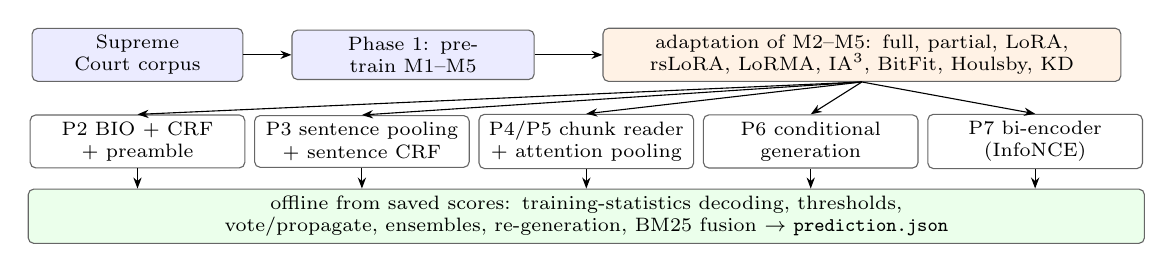
\begin{tikzpicture}[font=\scriptsize, >={Stealth[length=4pt]},
  box/.style={draw=black!60, rounded corners=2pt, align=center, inner sep=2.5pt, fill=#1}, box/.default=white]
\node[box=blue!8, text width=2.5cm] (corpus) at (-5.9, 0) {Supreme Court corpus};
\node[box=blue!8, text width=2.9cm] (p1) at (-2.4, 0) {Phase 1: pretrain M1--M5};
\node[box=orange!10, text width=6.4cm] (ad) at (3.3, 0) {adaptation of M2--M5: full, partial, LoRA, rsLoRA, LoRMA, IA$^3$, BitFit, Houlsby, KD};
\node[box, text width=2.55cm] (h2) at (-5.9, -1.1) {P2 BIO + CRF\\+ preamble};
\node[box, text width=2.55cm] (h3) at (-3.05, -1.1) {P3 sentence pooling + sentence CRF};
\node[box, text width=2.55cm] (h45) at (-0.2, -1.1) {P4/P5 chunk reader + attention pooling};
\node[box, text width=2.55cm] (h6) at (2.65, -1.1) {P6 conditional generation};
\node[box, text width=2.55cm] (h7) at (5.5, -1.1) {P7 bi-encoder (InfoNCE)};
\node[box=green!8, text width=14cm] (pp) at (-0.2, -2.05) {offline from saved scores: training-statistics decoding,
thresholds, vote/propagate, ensembles, re-generation, BM25 fusion $\to$ \texttt{prediction.json}};
\draw[->] (corpus) -- (p1); \draw[->] (p1) -- (ad);
\foreach \n in {h2,h3,h45,h6,h7} {\draw[->] (ad.south) -- (\n.north); \draw[->] (\n.south) -- (\n.south |- pp.north);}
\end{tikzpicture}
\caption{The system: every task model descends from my Phase~1 weights; decisions after the network are recomputed
offline from saved scores.}
\label{fig:overview}
\end{figure}

\subsection{Phase 2 --- Legal NER}\label{sec:p2}
Because spans require exact labels and character offsets, I used BIO tagging on overlapping 1{,}024-token windows
(stride 512) and reconstructed spans with the tokenizer's character offsets (Section~\ref{sec:prep}). I compared
softmax, BIO-constrained Viterbi and a linear-chain CRF~\cite{lafferty,lample}. A 256-token preamble gave later
windows access to the case header. At document level, \emph{vote} assigns repeated strings their majority label
and \emph{propagate} copies a predicted label to other occurrences, following InLegalNER~\cite{inlegalner}. I
dropped a greedy span ensemble because choosing it on only 10 validation documents led to overfitting.

\subsection{Phase 3 --- Rhetorical role prediction}\label{sec:p3}
I classified sentences in overlapping 1{,}024-token document windows so each could use its neighbours as context.
Mean-pooled sentence vectors fed a linear layer or a sentence-level CRF; Corporate Law and IT data were trained
together. I also decoded saved scores using training-role frequencies and transitions~\cite{menon,hybrid}, with
or without a position prior, and averaged runs in ensembles.

\subsection{Phase 4 --- Court judgment prediction}\label{sec:p4}
For each case, I encoded 512-token chunks and combined them with learned attention pooling. I compared reading
the head, middle and tail because outcomes usually appear near the end. Most runs used 10{,}000 cases; four M5
runs used all 31{,}677. The positive rate was 41\% in training and 50\% in development, so I compared argmax,
training-prior and development-fitted thresholds, both per run and in ensembles.

\subsection{Phase 5 --- Legal statute identification}\label{sec:p5}
I reused the Phase~4 reader with 100 sigmoid outputs and binary cross-entropy. Since statute names are masked,
the model must infer them from the facts; the first four 512-token chunks cover 78\% of documents. Output biases
start at the training log-odds. I compared global and per-statute thresholds, and always returned the most probable
statute.

\subsection{Phase 6 --- Abstractive summarization}\label{sec:p6}
I trained conditional language models to continue each document with its summary, using 1{,}024 document tokens
from the head and tail and up to 1{,}024 summary tokens. The M5 prefix-LM pretraining objective matches this setup;
79\% of reference summary bigrams also occur in the source document. I tested the permitted adapters and a
four-layer student, plus full fine-tuning for the GRU. Generation used greedy decoding with no repeated 4-grams;
I also tested a repetition penalty and consensus decoding.

\subsection{Phase 7 --- Prior case retrieval}\label{sec:p7}
The test set has 237 queries and 1{,}727 candidates. I encoded each case once with a bi-encoder~\cite{dpr} and
trained it with InfoNCE~\cite{infonce} and BM25~\cite{bm25} hard negatives, then fused its cosine scores with BM25.
Date and self-match rules remove impossible answers. Development data set the fusion weights and query penalty;
column normalisation adjusts each candidate's score across queries. Gradient caching made training practical
(Appendix~\ref{app:impl}).

\subsection{Final submitted system}
Table~\ref{tab:final} names the checkpoints behind each best submission; the repository notebooks are set to these runs.

\begin{table}[htbp]
\centering\small
\caption{Checkpoints behind the best submission of each phase.}
\label{tab:final}
\begin{adjustbox}{max width=\textwidth}
\begin{tabular}{cll}
\toprule
Phase & Checkpoint(s) & Decision layer / post-processing\\
\midrule
1 & Model 4 (\texttt{legal-modern-dec-101m}) & MBR over 14 decoded candidates, BERTScore utility\\
2 & \run{m5\_lorma\_crf\_pre} (M5, LoRMA, CRF, preamble 256) & CRF Viterbi + vote + propagate\\
3 & \run{m5\_\{lora,rslora,lorma,full\}\_crf} (M5) & CRF ensemble, prior + training-transition Viterbi\\
4 & \run{m5\_\{lora,rslora,lorma,full\}\_alldocs} (M5) & ensemble, last $8\times512$ tokens, dev-fitted threshold\\
5 & \run{m4\_full}, \run{m4\_lorma} (M4) & ensemble, per-statute thresholds\\
6 & \run{m4\_lora} (M4, LoRA) & greedy, no-repeat 4-grams, repetition penalty 1.15\\
7 & BM25 only (best model-based: ensemble of all six runs) & date/self rules, BM25 fusion, column normalisation, $p{=}0$\\
\bottomrule
\end{tabular}
\end{adjustbox}
\end{table}

% ============================================================
\section{Experiments and Implementation Details}
% ============================================================
\subsection{Compute and training protocol}
Training ran on Kaggle (two T4 GPUs); a laptop RTX~5050 served only inference and post-processing. Phase~1 used the
Hugging Face \texttt{Trainer}~\cite{hf}; each of Phases~2--7 has one PyTorch~\cite{pytorch} notebook with all its
experiments, training one run per GPU in parallel and writing logs, metrics, saved scores and submissions after every
run (a killed session loses at most one run); a 12-hour session held 5--8 runs of 6--192 minutes. Settings were
untuned starting values shared within a phase (Table~\ref{tab:hparams}): AdamW, linear warm-up and decay, weight decay
0.01, clipping 1.0, token-budget batches, bf16 autocast (Phases~2--5) or fp16 with a gradient scaler (6--7); the kept
epoch has the best validation metric (Phase~6: loss).

\begin{table}[htbp]
\centering\small
\caption{Hyperparameters of the final model in each phase (tok.\ = tokens per optimizer step).}
\label{tab:hparams}
\begin{adjustbox}{max width=\textwidth}
\begin{tabular}{lccccccc}
\toprule
Hyperparameter & P1 & P2 & P3 & P4 & P5 & P6 & P7 \\
\midrule
Parameters (M), trained & 101.3, all & 102.5, 1.13 & 102.4, 1.10$^a$ & 102.6, 1.28$^a$ & 101.6, all$^b$ & 102.4, 1.09 & 102.4, 1.11\\
Context length & 1024 & 1024 windows & 1024 windows & 1$\times$512 tail & 4$\times$512 head & 1024+1024 & 2$\times$512 head\\
Peak LR (backbone / adapter) & $6\!\times\!10^{-4}$ & $3\!\times\!10^{-5}$ / $3\!\times\!10^{-4}$ & same & same & same & $5\!\times\!10^{-5}$ / $3\!\times\!10^{-4}$ & $3\!\times\!10^{-5}$ / $3\!\times\!10^{-4}$\\
Batch $\times$ accum. & 8$\times$2 GPU$\times$4 (65k tok.) & 4 win.\ $\times$ 2 & 4k tok.\ $\times$ 2 & 4k tok.\ $\times$ 2 & 4k tok.\ $\times$ 2 & 4k tok.\ $\times$ 4 & 16 queries\\
Epochs (selected) & 1 (3.3k steps) & 8 (3) & 6 (3--5) & 3 (3) & 3 (3) & 2 (2) & 6 (6)\\
Dropout & none & 0.1 & 0.1 & 0.1 & 0.1 & --- & ---\\
Decoding / threshold & MBR (BERTScore) & CRF + vote/prop. & prior + Viterbi & dev threshold & per statute & greedy, ng4, rp 1.15 & rules + fusion\\
\bottomrule
\end{tabular}
\end{adjustbox}
\\[1pt]{\footnotesize $^a$LoRA member of the ensemble (also rsLoRA, LoRMA and full runs). $^b$\run{m4\_full}; its partner
\run{m4\_lorma} trains 1.38M. Warm-up 10\% of steps (Phase~6: 5\%); new layers use a learning rate of $10^{-3}$.}
\end{table}

\subsection{Local evaluation}
I evaluated on held-out data or official development sets and checked submissions with the official scorers.
My Phase~3 implementation matched the official score to six decimals. For decisions fitted on development data,
I also report two-fold cross-validation (CV), fitting on one half and scoring on the other across repeated splits.
Local estimates matched Codabench most closely in Phases~1, 6 and~7. Phase~3 was the main exception: two roles
were absent from development, lowering its macro-F1. Rescaling the 11 observed roles by $13/11$ removes most of
the gap. Phase~4 CV estimates were within 0.017 of test for the reported choices, except for a high-scoring run
selected from about a hundred candidates.

\subsection{Ablations and controlled comparisons}
Table~\ref{tab:ablations} changes one factor at a time on validation data; complete run tables are in the appendix.

\begin{table}[htbp]
\centering\scriptsize
\caption{Controlled comparisons (one factor changed; validation scores; CV = 2-fold cross-validated).}
\label{tab:ablations}
\begin{adjustbox}{max width=\textwidth}
\begin{tabular}{clll}
\toprule
Phase & Factor & Setting compared & Score\\
\midrule
1 & architecture (same data) & M1 $\to$ M2 $\to$ M4 (val.\ loss, nats/token) & 4.742 $\to$ 3.007 $\to$ 2.992\\
1 & decoding (M4 fixed) & greedy $\to$ + 3-gram block $\to$ + 4-gram, rp 1.2 $\to$ MBR (pseudo-val.) & 0.8048 $\to$ 0.8351 $\to$ 0.8372 $\to$ 0.8419\\
2 & output layer (M4 LoRMA) & softmax $\to$ constrained Viterbi $\to$ CRF & 0.3202 $\to$ 0.4131 $\to$ 0.4502\\
2 & preamble context (M4 LoRMA CRF) & none $\to$ 256 tokens & 0.4502 $\to$ 0.4561\\
2 & document rules (M4 LoRMA CRF) & none $\to$ vote / propagate / both & 0.4502 $\to$ 0.4591 / 0.4739 / 0.4813\\
2 & distillation (4-layer student) & no teacher $\to$ teacher & 0.2695 $\to$ 0.2841\\
3 & output layer (M5 LoRA) & linear $\to$ sentence CRF & 0.4407 $\to$ 0.4685\\
3 & decoding (M5 CRF ensemble) & own Viterbi $\to$ prior + training Viterbi & 0.453 $\to$ 0.471\\
3 & distillation & 10-layer teacher $\to$ 4-layer student (training minutes) & 0.442 (46.6) $\to$ 0.347 (17.5)\\
4 & training data (M5 rsLoRA) & 10k $\to$ 31.7k cases & 0.6615 $\to$ 0.7087\\
4 & section read (8 runs) & head / middle / head+tail / tail & 0.53--0.57 / 0.50--0.58 / 0.61--0.64 / 0.62--0.66\\
4 & distillation & teacher \run{m5\_full} $\to$ 4-layer student (training minutes) & 0.6528 (69) $\to$ 0.6503 (26)\\
5 & threshold (M4 ensemble, CV) & one global $\to$ per statute & 0.3546 $\to$ 0.3673\\
5 & method (M5, global threshold) & full / LoRMA / partial / KD student & 0.3532 / 0.3292 / 0.3364 / 0.3461\\
6 & document part read (M5 LoRMA) & head 1024 $\to$ head+tail 1024 (BERTScore) & 0.8337 $\to$ 0.8361\\
6 & distillation & teacher \run{m5\_lorma} $\to$ 4-layer student & 0.8361 $\to$ 0.8232\\
7 & training (M5 LoRMA, raw ranking) & Phase~1 model (0-shot) $\to$ fine-tuned & 0.2424 $\to$ 0.3091\\
7 & post-processing (M5 LoRMA) & raw $\to$ + BM25, no column term $\to$ full (CV) & 0.3091 $\to$ 0.3413 $\to$ 0.4308\\
\bottomrule
\end{tabular}
\end{adjustbox}
\end{table}

% ============================================================
\section{Results}
% ============================================================
Table~\ref{tab:results} compares local and Codabench scores; full run tables are in Appendices~\ref{app:p1}--\ref{app:p7}.
Figure~\ref{fig:curves} shows selected learning curves. Macro-F1 also hides large class differences: the best Phase~2
F1 ranges from 0.11 (appellant) to 0.93 (date), and Phase~3 from 0.27 (\emph{None}) to 0.82 (\emph{Statute}).
Phase~5 statute F1 ranges from 0.05 to 0.83 and rises with training frequency ($\rho=0.57$); the rarest quarter
averages 0.25, against 0.51 for the most frequent.

\begin{table}[htbp]
\centering\small
\caption{Best submission per phase and model: its local score (validation; 2-fold CV where a decision was fitted on the
validation data) / Codabench. n/r = not recorded; --- = no run.}
\label{tab:results}
\begin{adjustbox}{max width=\textwidth}
\begin{tabular}{llcccc}
\toprule
Phase & Metric & M2 & M3 & M4 & M5\\
\midrule
1 & BERTScore F1 & --- / 0.8087 & --- / 0.7874 & 0.8419 / \best{0.8407} & --- / 0.8300\\
2 & strict macro-F1 & 0.2899 / 0.3416 & 0.1906 / n/r & 0.4561$^\dagger$ / 0.4754 & 0.4797$^\dagger$ / \best{0.5122}\\
3 & macro-F1 & 0.439 / 0.4952 & 0.350 / 0.3338 & 0.441 / 0.5245 & 0.471 / \best{0.5713}\\
4 & macro-F1 & 0.7188$^\ddagger$ / 0.6889 & 0.5927 / n/r & 0.6787 / n/r & 0.7521 / \best{0.7609}\\
5 & macro-F1 & 0.3387 / n/r & 0.2446 / n/r & 0.3673 / \best{0.3664} & 0.3624 / 0.3588\\
6 & BERTScore F1 & 0.8377 / 0.8329 & 0.8033 / n/r & 0.8423 / \best{0.8381} & 0.8361 / 0.8322\\
7 & Micro-F1@7 & --- & 0.4263 / n/r & 0.4280 / 0.4253 & 0.4317 / 0.4300\\
\bottomrule
\end{tabular}
\end{adjustbox}
\\[1pt]{\footnotesize $^\dagger$before vote/propagate. $^\ddagger$fixed rule (no CV needed). Phase~7: BM25 with the same
post-processing 0.4249 (CV) / \best{0.4318}; six-run ensemble 0.4245 / 0.4318 (both $p{=}0$).}
\end{table}

\noindent There was no single winning backbone across all seven tasks. M5 with a four-run CRF ensemble and
training-prior/transition Viterbi decoding led Phase~3 at 0.5713; M5 ensembles with more training cases and longer
tail reading led Phase~4 at 0.7609; and M4 was strongest in pretraining, statute identification and summarisation.
In retrieval, task-aware post-processing was decisive: BM25 with date/self rules and cross-query column
normalisation reached 0.4318, matching the six-run ensemble. In these experiments, data access and task-specific
decision structure often mattered more than adding model capacity.

% ============================================================
\section{Error Analysis and Discussion}
% ============================================================
I rely most on controlled comparisons and cross-validation. Codabench scores show how well local estimates
transferred to test; they are not used to select methods. Validation is especially small in Phases~2, 3 and~7, so
differences below about 0.01 are meaningful only when they recur across runs.

\subsection{Phase-wise failure modes}
\textbf{Phase 1: repetition.} Plain greedy decoding repeats 69\% of word 4-grams. A 4-gram block and repetition
penalty raise distinct bigrams from 0.27 to 0.93, but ROUGE-L falls from 0.1995 to 0.1865. The model becomes less
repetitive, not better informed.

\textbf{Phase 2: role-defined entities and boundaries.} Appellants, respondents, counsel and witnesses reach only
0.11--0.24 F1; dates and statutes reach 0.93 and 0.85. The weak labels are all person names, often identified by a
role in the header rather than near later mentions. Half of all mentions lie beyond token 1{,}024. Exact offsets
also matter: trimming spans raises the round-trip ceiling from 0.605 to 0.979.

\textbf{Phase 3: speaker and rhetorical function.} The main confusions are petitioner arguments labelled as
respondent arguments (136 development sentences) and facts labelled as reasoning (75). The \emph{None} class reaches
0.27 F1; Corporate Law is harder than IT across all 17 runs (0.362 vs.\ 0.465).

\textbf{Phase 4: prior shift and less explicit outcomes.} Acceptance is 41.4\% of training labels and 50\% of
development labels, so models under-predict it unless the threshold is adjusted. Explicit outcome words also occur
less often in test tails (13\%) than in training tails (24\%), making the test cases harder for models that rely on
the disposition sentence.

\textbf{Phase 5: rare statutes.} Two statutes remain below 0.1 F1. The rarest quarter averages 0.25, against 0.51
for the most frequent. Since macro-F1 weights each label equally, the tuned thresholds favour recall; the system
predicts 5.2 statutes per development document, compared with 3.9 gold.

\textbf{Phase 6: short summaries and truncation.} Submitted M4 summaries average 535 words, against 852 for the
references; 11\% reach the length cap. BERTScore compares only about the first 400 words, so a good score says
little about later content or factual accuracy.

\textbf{Phase 7: fixed-size retrieval and generic candidates.} Returning exactly seven cases caps a perfect ranker
at 0.618 on development because relevance counts vary. Generic candidates that score well for many queries are
another problem; column normalisation reduces this hub effect. Post-processed systems score 0.426--0.433.

\subsection{What the metrics do not measure}
Strict span F1 penalises even a one-character offset error. Macro-F1 gives rare labels the same weight as common
ones, so thresholds matter. Truncated BERTScore rewards similarity in the opening of a summary but does not check
whether later statements are true. Micro-F1@7 always requires seven answers, regardless of how many are relevant.
None of these metrics measures confidence calibration, which a lawyer would need to judge whether to trust a result.

\subsection{Limitations and what I would do next}
Several limits affect these results. Phases~2--3 validate on 10 documents and Phase~7 on 118 queries; each run used
one seed, and hyperparameters were not tuned. The models saw about two training tokens per parameter and read at
most 1{,}024 tokens, while many judgments are much longer. Phase~1's pseudo-validation prompts came from the test
prompts, Phase~6 has no official development set, the Phase~7 M2 runs did not complete, and no legal expert reviewed
the outputs.

Two roles are missing from Phase~3 development. Since the scorer averages all 13 roles and assigns zero to absent
ones, its development score is reduced by the factor $11/13$. Rescaling by $13/11$ explains most of the 0.05--0.10
Codabench advantage seen in nine of ten submissions. In Phase~4, CV estimates were within 0.017 of test except for
\run{m2\_lorma}, whose development score (0.7188) had been selected from about a hundred candidates and fell to
0.6889 on test.

My next steps would be to run three seeds per phase, use the unused High Court and Tribunal data for continued pretraining,
test bidirectional continuation of M4, tune LoRMA's learning rate against LoRA, and extend context beyond 1{,}024
tokens. Phase-specific tests include a sentence-only Phase~3 run, Phase~7 cross-encoder reranking, summary length
control, and submitting the Phase~1 MBR setting.

\subsection{Surprising findings}
M5 scored below M4 as a language model but performed better in the reading tasks submitted by both. In Phase~3,
role priors and training transitions raised the score from 0.504 to 0.571. In Phase~7, BM25 with post-processing
matched the six-run ensemble at 0.4318. A four-layer student also retained 99.6\% of its Phase~4 teacher's score
while taking 38\% as long to train.

% ============================================================
\section{Conclusion}
% ============================================================
I built a compact legal-language system from scratch using the official data. With roughly two training tokens per
parameter and documents longer than the 1{,}024-token context, data and context were bigger constraints than model
size. The strongest gains often came from task-specific methods: CRFs and training statistics for sequences,
thresholds for imbalanced labels, and normalisation for retrieval. M5's bidirectional pretraining also transferred
well to reading tasks.

Local scores were useful when based on held-out data or cross-validation; the largest test gaps had identifiable
causes. Still, rare entity and statute predictions remain unreliable, and a high truncated BERTScore does not
guarantee a factually correct summary. No legal expert reviewed the outputs, so the system should be treated as
decision support, not legal advice. Code and documentation:
\url{https://github.com/D3bug1t/LLM-Pretraining-PostTraining-Extrinsic-Instrinsic-Evals}.

% ============================================================
\clearpage
\section*{LLM Usage Declaration}
% ============================================================
Completing this section is mandatory. Inconsistent answers relative to the code and the prose will be treated as an integrity issue.

\medskip
\noindent
\textbf{Q1.} Which Large Language Model(s), if any, did you use while completing the competition or writing this report? Give model name and vendor (e.g., none / ChatGPT-4.x / Gemini~x / Claude~x / Grok / Copilot / other). \\[0.6em]
Answer: Claude Opus 5.5 generated the separate LLM-based analysis document from my project results. GitHub Copilot
in VS Code assisted with integrating and editing this report; neither was part of the competition system or used to
produce the experimental results.

\medskip
\noindent
\textbf{Q2.} For each row, mark Yes or No and state the purpose in one short phrase. ``Yes'' is acceptable only for the uses permitted by the capstone document.

\begin{table}[H]
\centering
\begin{tabular}{>{\raggedright\arraybackslash}p{4.6cm}|c|>{\raggedright\arraybackslash}p{7.2cm}}
\toprule
Part & Used LLM? & Purpose of using the LLM \\
\midrule
Understanding concepts / papers & No & --\\
Ideation / brainstorming at a high level & Yes & Claude's separate analysis suggested follow-up experiments\\
Debugging small ancillary snippets & No & --\\
Plotting / visualization code & Yes & Claude analysis figures comparing calibration and distillation\\
Grammar / writing style of the report & Yes & Claude analysis document; Copilot report editing\\
Report structure / section wording & Yes & Claude analysis document; Copilot integration\\
Designing the model architecture & No & --\\
Hyperparameter search / tuning & No & No LLM-based tuning; settings were not searched\\
Analysis of results / conclusions & Yes & Claude wrote the separate analysis from my scores and run records\\
Writing the core training / inference code & No & --\\
Other (specify) & No & --\\
\bottomrule
\end{tabular}
\end{table}

\medskip
\noindent
\textbf{Q3.} Did you refer to sources other than lecture slides and an LLM?
If yes, list them (papers, blogs, GitHub repositories, textbooks, official starter notebook, evaluation scripts). These must also appear in the bibliography when they influenced the method. \\[0.4em]
Answer: Yes. I used the papers cited in the bibliography, the official course starter code and data, and the
official evaluation scripts for scoring and format validation.

\medskip
\noindent
\textbf{Q4.} Apart from any permitted LLM use, what was \emph{your} contribution? In 8--12 sentences describe your own understanding, architecture decisions, implementation, experiments, and analysis. Name at least two things you tried that failed and what you concluded from them.

\medskip
\noindent
I designed and trained five language models from scratch on the official Supreme Court corpus, comparing decoder
architectures and a prefix-LM under the project compute limits. I built a byte-level BPE tokenizer and an
offset-preserving version for exact named-entity spans. For Phases~2--7, I adapted the pretrained checkpoints with
full fine-tuning, parameter-efficient methods, task-specific heads and distillation, then evaluated the runs on
held-out or official development data. I implemented task-specific post-processing, including CRF and
training-statistic decoding, threshold selection, document rules, and lexical/dense retrieval fusion. I also
checked submissions with the official evaluation scripts and investigated gaps between local and Codabench
scores. In Phase~1, MBR improved pseudo-validation but I did not submit it, so its hidden-test performance remains
unknown. In Phase~4, head-only reading was weaker than reading the tail, consistent with the decision appearing
near the end of judgments. The four-layer student was substantially weaker than its teacher in Phases~2--3, though
it retained nearly all the teacher's Phase~4 score with much less training time. I drew the experimental results
and conclusions from my own runs; Claude Opus 5.5 wrote the separate analysis document based on those results.

\bibliographystyle{ieeetr}
\bibliography{references}

% ============================================================
\clearpage
\appendix
\section*{Appendix}
The appendix holds the complete per-phase tables referenced from the main text.

\section{Learning curves and per-class breakdowns}\label{app:curves}
\begin{figure}[H]
\centering
\begin{subfigure}[t]{0.32\textwidth}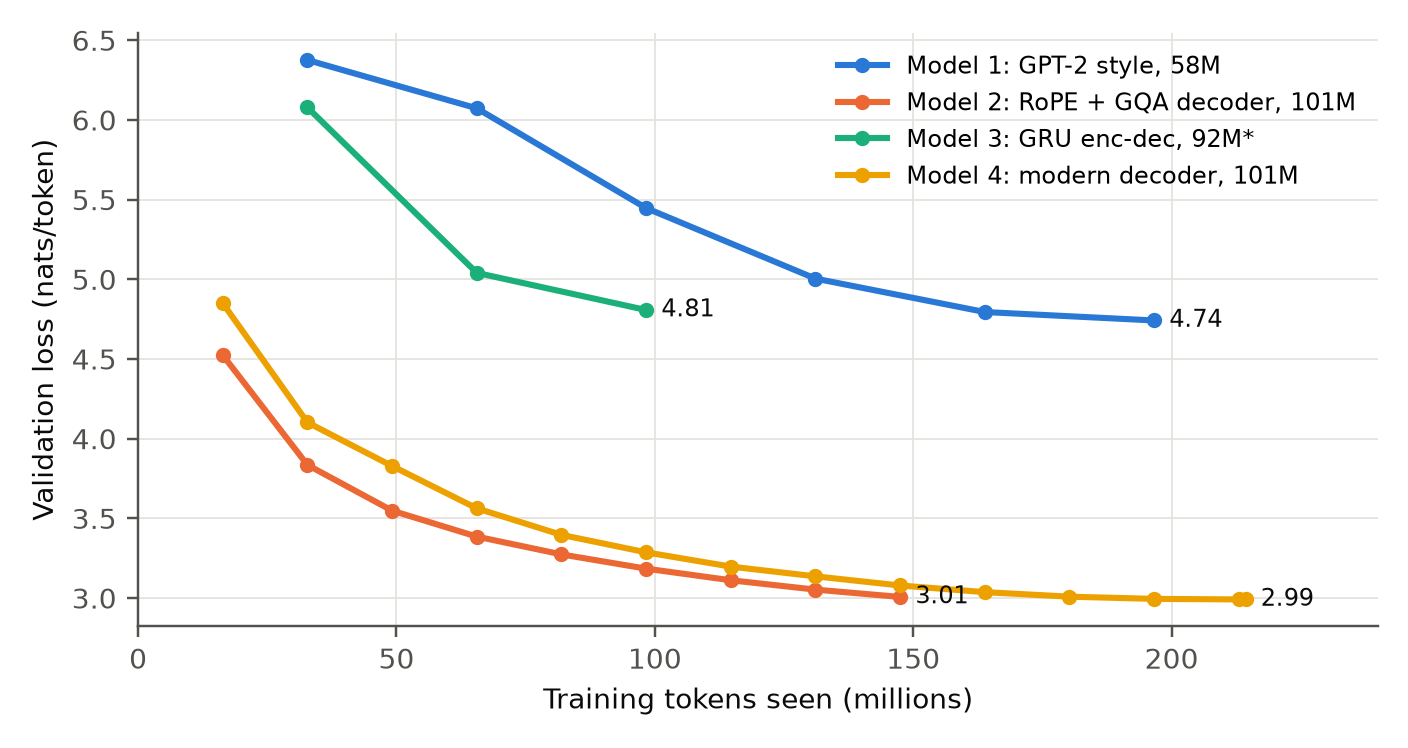
\includegraphics[width=\textwidth]{val_loss.png}\caption{Phase 1 validation loss vs.\ training tokens.}\end{subfigure}\hfill
\begin{subfigure}[t]{0.32\textwidth}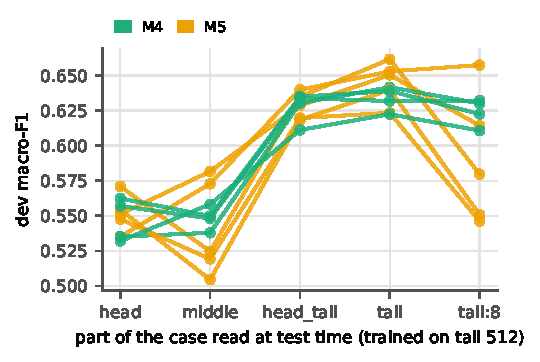
\includegraphics[width=\textwidth]{p4_sections.pdf}\caption{Phase 4: the eight 10k-case M4/M5 runs (trained on the last 512 tokens) reading other parts at test time.}\end{subfigure}\hfill
\begin{subfigure}[t]{0.32\textwidth}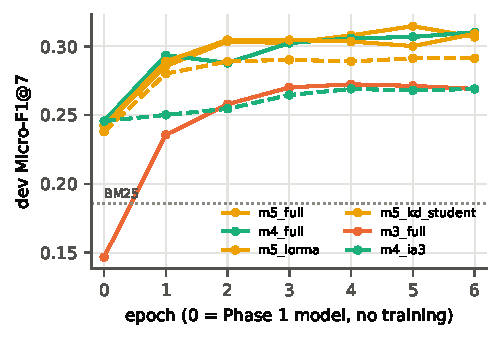
\includegraphics[width=\textwidth]{p7_epochs.pdf}\caption{Phase 7 dev Micro-F1@7 per epoch (0 = untrained Phase~1 model; dashed: KD, IA$^3$).}\end{subfigure}
\caption{Learning curves and the Phase~4 reading analysis.}
\label{fig:curves}
\end{figure}

\begin{figure}[H]
\centering
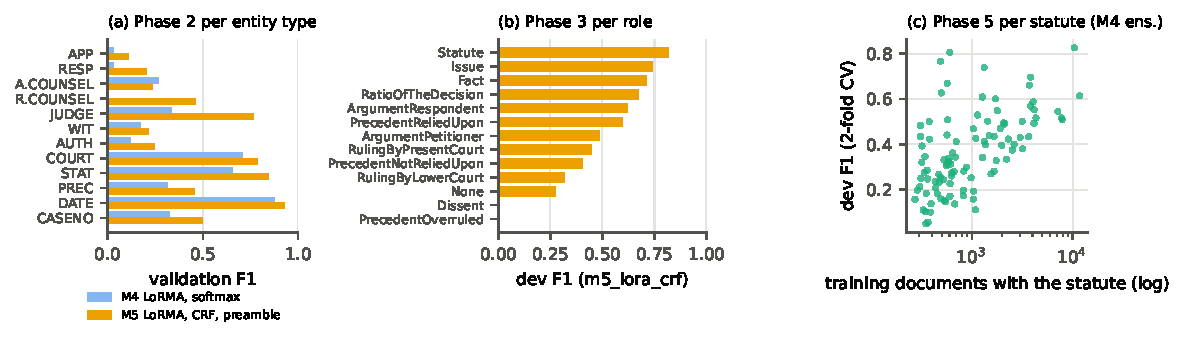
\includegraphics[width=\textwidth]{per_class.pdf}
\caption{Per-class breakdowns: (a) Phase~2 validation F1 per entity type, first and best system; (b) Phase~3 dev F1 per
role of \run{m5\_lora\_crf} (\emph{Dissent} and \emph{PrecedentOverruled} do not occur in dev); (c) Phase~5 dev F1 per
statute against its training frequency (M4 ensemble, per-statute thresholds fitted on the other half of dev).}
\label{fig:perclass}
\end{figure}

\section{Architecture and design rationale}\label{app:arch}
This appendix summarises the architecture and task-layer trade-offs behind the experiments.

\subsection{The constraints that shaped the choices}
The model budget was 50--300M parameters; I chose about 100M so models could be trained on two T4 GPUs within a
12-hour session. The Supreme Court corpus contains about 275M tokens, or roughly two tokens per parameter for one
epoch, so throughput mattered. Phase~1 required continuation of a 512-word passage, while later tasks required the
same weights to handle tagging, classification, generation and retrieval on much longer documents. I designed the
model sequence to test these trade-offs (Section~\ref{sec:p1}).

\subsection{The five Phase-1 models}
\begin{table}[H]
\centering\scriptsize
\caption{Phase-1 architectures: the question each one asked, its advantages and drawbacks, and the outcome
(validation loss in nats/token / Codabench BERTScore; downstream results from Table~\ref{tab:results}).}
\label{tab:archwhy}
\begin{adjustbox}{max width=\textwidth}
\begin{tabular}{>{\raggedright\arraybackslash}p{1.2cm}>{\raggedright\arraybackslash}p{3.2cm}>{\raggedright\arraybackslash}p{3.6cm}>{\raggedright\arraybackslash}p{3.6cm}>{\raggedright\arraybackslash}p{3.4cm}}
\toprule
Model & Question asked & Advantages & Drawbacks & Outcome\\
\midrule
M1 GPT-2 style, 58M &
Does the starter pipeline work end to end, and where does it fail? &
Simple, known to train stably; 2{,}048-token context; quick to build. &
Absolute sinusoidal positions; full multi-head KV cache; biases and LayerNorm/GELU; only 58M of the 100M budget; no
repetition control. &
4.742 / 0.7830. Loops such as ``to the High Court to the High Court''. Not carried forward.\\
\addlinespace
M2 RoPE + GQA, 101M &
Do relative positions, shared key/value heads and the full parameter budget help? &
RoPE encodes the offset between tokens, which suits a passage starting at an arbitrary point; GQA stores 3$\times$
fewer keys/values, so decoding is faster. &
Still LayerNorm/GELU with biases; small batches (16k tokens); stopped at 74\% of the epoch (147M tokens). &
3.007 / 0.8087. Downstream: best single 10k-case run in Phase~4 (0.6831); close second in Phase~6.\\
\addlinespace
M3 GRU enc.--dec., 92M &
Can the encoder--decoder family, with a bidirectional encoder and attention, compete at the same size? &
The encoder reads the whole prompt in both directions; constant memory per generated token; well understood
(Assignment~2). &
The recurrence runs one time step at a time, so it trains slowly (98M tokens in budget); a fixed-size state summarises
the context; more than half of the encoder is embeddings; no linear layers, so LoRA-type methods do not apply. &
4.808$^*$ / 0.7874. Weakest model in every downstream phase (e.g.\ Phase~5 dev 0.2105 vs.\ 0.3535).\\
\addlinespace
M4 modern decoder, 101M &
With M2's shape fixed, does the current open-model recipe give a better model from the same budget? &
RMSNorm and SwiGLU give more quality per parameter; no biases; scaled residual initialisation allows a higher learning
rate; 4$\times$ larger batches, made possible by a chunked loss that saves memory, raise throughput, so it completed a full epoch (214M tokens). &
Causal attention only, so reading tasks need a mask change at fine-tuning; context 1{,}024 tokens. &
\textbf{2.992 / 0.8324} (0.8407 with MBR decoding). Best language model; best in Phases~1, 5 and~6.\\
\addlinespace
M5 prefix-LM, 101M &
With M4's network fixed, does reading the prompt bidirectionally during pretraining help? &
Pretraining matches the downstream pattern ``read a document whole, then decide or write''; less mismatch when the
causal mask is removed for fine-tuning. &
Loss only on the continuation ($\approx$65\% of tokens supervised); needs an explicit mask per example, so the fused
causal attention kernel cannot be used. &
--- / 0.8300, slightly below M4 as a language model. Best in Phases~2, 3 and~4; best model-based in Phase~7.\\
\bottomrule
\end{tabular}
\end{adjustbox}
\\[1pt]{\footnotesize $^*$Loss on the continuation only; not comparable with the decoders.}
\end{table}

\textbf{What the model comparisons show.} M3 processed 98M tokens, less than half of M4's 214M, because its GRU
runs sequentially. This likely contributed to its weaker results; its lack of linear layers also ruled out the
adapter methods used with the decoders. The M1-to-M2 comparison changes several factors at once, so it cannot
isolate the effect of RoPE or GQA. M2 and M4 have the same shape, but M4 processed 45\% more tokens; its better
loss and Codabench score reflect both the recipe and the additional training it enabled.

M5's Phase~1 score was slightly below M4's, but it led Phases~2--4 and the learned Phase~7 retriever. One possible
reason is that M5's bidirectional prompt training better matches downstream reading tasks. This was not tested
directly. Where M4 led, the margins were small: 0.0004 for Phase~5 full fine-tuning and 0.0017 in held-out Phase~6
BERTScore.

\subsection{Attention mechanisms}
\begin{table}[H]
\centering\scriptsize
\caption{Attention used by each Phase-1 model. KV cache = numbers stored per generated token over all layers.}
\label{tab:attn}
\begin{adjustbox}{max width=\textwidth}
\begin{tabular}{llccllr}
\toprule
Model & Mechanism & Q / KV heads & $d_h$ & Mask & Positions & KV cache\\
\midrule
M1 & multi-head self-attention & 8 / 8 & 70 & causal & sinusoidal, added to embeddings & 8{,}960\\
M2 & grouped-query self-attention & 12 / 4 & 64 & causal & RoPE on $q,k$ & 5{,}120\\
M3 & Bahdanau additive cross-attention (no self-attention) & 1 (dim 256) & --- & prompt padding & GRU recurrence & ---\\
M4 & grouped-query self-attention & 12 / 4 & 64 & causal & RoPE on $q,k$ & 5{,}120\\
M5 & grouped-query self-attention & 12 / 4 & 64 & bidirectional over prompt, causal after & RoPE on $q,k$ & 5{,}120\\
\bottomrule
\end{tabular}
\end{adjustbox}
\end{table}
\noindent GQA lets query head $i$ use key/value group $\lfloor i/3\rfloor$. This keeps 12 query views and cuts the
cache by $3\times$ against 12-head attention, which kept the cache small for the 28-setting decoding study and the MBR
candidate pools on a laptop GPU. RoPE rotates query and key pairs by angles proportional to position, so $q_m^\top k_n$ depends only on
$m-n$. With left-padded batches, each row's positions start at its first real token. In Phase~6 the same rotation was
extended from 1{,}024 to 2{,}048 positions without retraining from scratch, which a learned table of absolute positions
would not allow.

\subsection{Task layers: what I chose and what I did not}
\begin{table}[H]
\centering\scriptsize
\caption{Task-layer choices per phase, the alternatives considered, the reasons, and the known weaknesses.}
\label{tab:headwhy}
\begin{adjustbox}{max width=\textwidth}
\begin{tabular}{>{\raggedright\arraybackslash}p{0.6cm}>{\raggedright\arraybackslash}p{3.1cm}>{\raggedright\arraybackslash}p{3.1cm}>{\raggedright\arraybackslash}p{4.4cm}>{\raggedright\arraybackslash}p{3.6cm}}
\toprule
Phase & Chosen & Alternatives & Why chosen & Weakness\\
\midrule
2 & BIO tagging with a CRF on overlapping 1{,}024-token windows, 256-token preamble & softmax tagging; constrained
Viterbi; span enumeration & The CRF scores whole tag sequences, so spans are valid and transitions are learned; the parallel partition
function made it as cheap as softmax (0.036\,s per batch); span enumeration over 4{,}498-word documents is costly &
A boundary error still costs the whole span; rare party labels stay weak (Fig.~\ref{fig:perclass}a)\\
\addlinespace
3 & Mean-pooled sentence vectors from document windows, linear or sentence-CRF output & one sentence per input;
a second hierarchical encoder & Neighbouring sentences are visible to the encoder; the CRF models role order; no extra
network to train & Only 10 dev documents to compare variants\\
\addlinespace
4 & $K$ chunks of 512 tokens, attention pooling, section chosen by experiment & truncation to the first 512 tokens;
reading the whole case & Cost grows linearly with $K$; the section can be changed at test time without retraining & Chunks do not see
each other; long cases are read only in part\\
\addlinespace
5 & Same reader, 100 sigmoids with log-odds bias, per-statute thresholds & softmax over label sets; one classifier per
statute & One shared encoder for all labels; rare statutes start calibrated & Rare statutes remain hard (F1 0.25 in the
rarest quarter)\\
\addlinespace
6 & Decoder as conditional LM on \texttt{[doc] <s> [summary]} & encoder--decoder (only M3); extractive selection &
Reuses the pretraining objective directly, with no new parameters except the adapter & Reads 1{,}024 tokens of a
median 3{,}146-word document; positions extended beyond pretraining\\
\addlinespace
7 & Bi-encoder, InfoNCE with BM25 hard negatives, fused with BM25 & cross-encoder re-ranking; BM25 only & One vector per
case scores all 409k test pairs cheaply; BM25 adds exact lexical matches & Reads only the first $2\times512$ tokens; 827
training queries\\
\bottomrule
\end{tabular}
\end{adjustbox}
\end{table}

\subsection{Adaptation techniques: advantages, drawbacks and my evidence}\label{app:techs}
\begin{table}[H]
\centering\scriptsize
\caption{Adaptation techniques (parameters trained for a 101M decoder), with evidence from my runs.}
\label{tab:techwhy}
\begin{adjustbox}{max width=\textwidth}
\begin{tabular}{>{\raggedright\arraybackslash}p{1.4cm}>{\raggedright\arraybackslash}p{2.9cm}>{\raggedright\arraybackslash}p{3.1cm}>{\raggedright\arraybackslash}p{3.1cm}>{\raggedright\arraybackslash}p{4.4cm}}
\toprule
Technique & What is trained & Advantages & Drawbacks & Evidence from my runs\\
\midrule
Full & all weights (101M) & Most capacity; reference point & Memory for optimizer state; may forget pretraining on
small data & Best single run in Phase~5 (M4 0.3535, M5 0.3531) and Phase~7 raw (M5 0.3146)\\
\addlinespace
Partial & top 5 of 10 layers (31.7M) & Keeps low layers as pretrained; cheaper & Lower layers cannot adapt & Phase~5:
0.3364, between LoRMA (0.3292) and full (0.3531) on M5\\
\addlinespace
LoRA & $W_0x+\frac{\alpha}{r}BAx$, $r{=}8$ ($\approx$1.1M) & 1\% of the parameters; base weights shared & Scale
$\alpha/r$ shrinks the update as $r$ grows & Within 0.01--0.02 of full in Phases~3--4 (e.g.\ M5 Phase~3: 0.441 vs.\
0.442)\\
\addlinespace
rsLoRA & as LoRA, scale $\alpha/\sqrt r$ & Update size stable in $r$ & One more scale choice & Higher than LoRA in 5 of 8
paired runs (Phases~3--4); best Phase~4 single run (0.7087)\\
\addlinespace
LoRMA & $(I+\frac{\alpha}{r}BA)W_0x$ ($\approx$1.1M) & Re-mixes the pretrained layer's outputs; same cost as LoRA via
$z+\frac{\alpha}{r}B(Az)$ & The update is tied to $W_0$'s output space & Lowest of the low-rank methods on M5 in Phases~3--4 and below full in Phase~5;
still the best Phase~2 submission (M5 LoRMA + CRF, 0.5122)\\
\addlinespace
IA$^3$ & per-channel scales (0.03M) & Smallest update & Little capacity & Phase~7: 0.2690 vs.\ 0.3102 for full M4\\
\addlinespace
BitFit & biases (0.08M on M3) & Tiny; applies to the GRU & Little capacity & Phase~2 M3: 0.1149 vs.\ 0.1906 full\\
\addlinespace
Houlsby & bottleneck layers $768{\to}64{\to}768$ (2.0M) & New capacity in series & Adds inference layers & Phase~6:
0.8377 held-out, within 0.0001 of M4 LoRA\\
\addlinespace
KD & 4-layer student (63.6M) on $(1-\lambda)\mathcal L+\lambda T^2\mathrm{KL}$ & $\approx$2.6$\times$ faster
training & Needs a teacher run first; loses depth & Student/teacher: Phase~4 99.6\%, Phase~5 98.0\%, Phase~7 94\%,
Phase~2 82\%, Phase~3 78\% of the teacher's score; Phase~2 student beats its no-teacher control (0.2841 vs.\ 0.2695)\\
\bottomrule
\end{tabular}
\end{adjustbox}
\end{table}

\section{Phase 1 details}\label{app:p1}
\begin{table}[H]
\centering\small
\caption{Phase 1 decoding on Model 4: pseudo-validation vs.\ Codabench BERTScore for the submitted settings.}
\label{tab:calib}
\begin{tabular}{lccc}
\toprule
Decoding & Pseudo-val & Codabench & $\Delta$\\
\midrule
$T$=0.1, top-$p$ 0.95, 4-gram block (notebook default) & 0.8327 & 0.8324 & $-0.0003$\\
Top-$p$ ($T$=0.7, $p$=0.9), 3-gram, rp 1.1 & 0.8355 & 0.8343 & $-0.0012$\\
Beam 4, 3-gram block & 0.8353 & 0.8345 & $-0.0008$\\
Greedy, 4-gram block, rp 1.1 & 0.8369 & 0.8352 & $-0.0017$\\
Greedy, 4-gram block, rp 1.2 & 0.8372 & 0.8363 & $-0.0009$\\
MBR, ROUGE-L utility, 14 candidates & 0.8393 & 0.8379 & $-0.0014$\\
MBR, BERTScore utility, 14 candidates & \best{0.8419} & \best{0.8407} & $-0.0012$\\
\bottomrule
\end{tabular}
\end{table}

\begin{table}[H]
\centering\small
\caption{Selected Phase 1 pseudo-validation results (300 prompts) with the secondary metrics; rep-4 = share of
repeated word 4-grams, dist-2 = share of distinct bigrams.}
\begin{tabular}{lccccc}
\toprule
Strategy & BERTScore & ROUGE-L & BLEU-4 & rep-4 & dist-2\\
\midrule
Greedy, no blocking & 0.8048 & 0.1898 & 0.0359 & 0.693 & 0.267\\
Greedy, 3-gram block & 0.8351 & 0.2046 & 0.0576 & 0.000 & 0.807\\
Greedy, 6-gram block & 0.8295 & 0.2055 & 0.0529 & 0.174 & 0.592\\
Greedy, 4-gram, rp 1.1 & 0.8369 & 0.1995 & 0.0634 & 0.000 & 0.831\\
Greedy, 4-gram, rp 1.2 & 0.8372 & 0.1865 & 0.0533 & 0.000 & 0.931\\
Top-$p$ $T$=0.9, 4-gram & 0.8318 & 0.1891 & 0.0406 & 0.000 & 0.887\\
Beam 4, 3-gram block & 0.8353 & \best{0.2069} & \best{0.0673} & 0.000 & 0.872\\
Contrastive $\alpha$=0.6 & 0.8263 & 0.1934 & 0.0412 & 0.029 & 0.869\\
MBR, utility ROUGE-L & 0.8393 & 0.2057 & 0.0655 & --- & ---\\
MBR, utility BERTScore & \best{0.8419} & 0.2041 & 0.0636 & --- & ---\\
\bottomrule
\end{tabular}
\end{table}

\begin{table}[H]
\centering\small
\caption{Phase 1 training runs (tokens per optimizer step, tokens seen, peak learning rate).}
\begin{tabular}{lrrr}
\toprule
Model & Tokens/step & Tokens & Peak LR\\
\midrule
M1 & 32{,}768 & 200M & $3\times10^{-4}$\\
M2 & 16{,}384 & 147M & $3\times10^{-4}$\\
M3 & 16{,}384 & 98M & $1\times10^{-3}$\\
M4 & 65{,}536 & 214M & $6\times10^{-4}$\\
M5 & 65{,}536 & --- & $6\times10^{-4}$\\
\bottomrule
\end{tabular}
\end{table}

\begin{figure}[H]
\centering
\begin{subfigure}[t]{0.49\textwidth}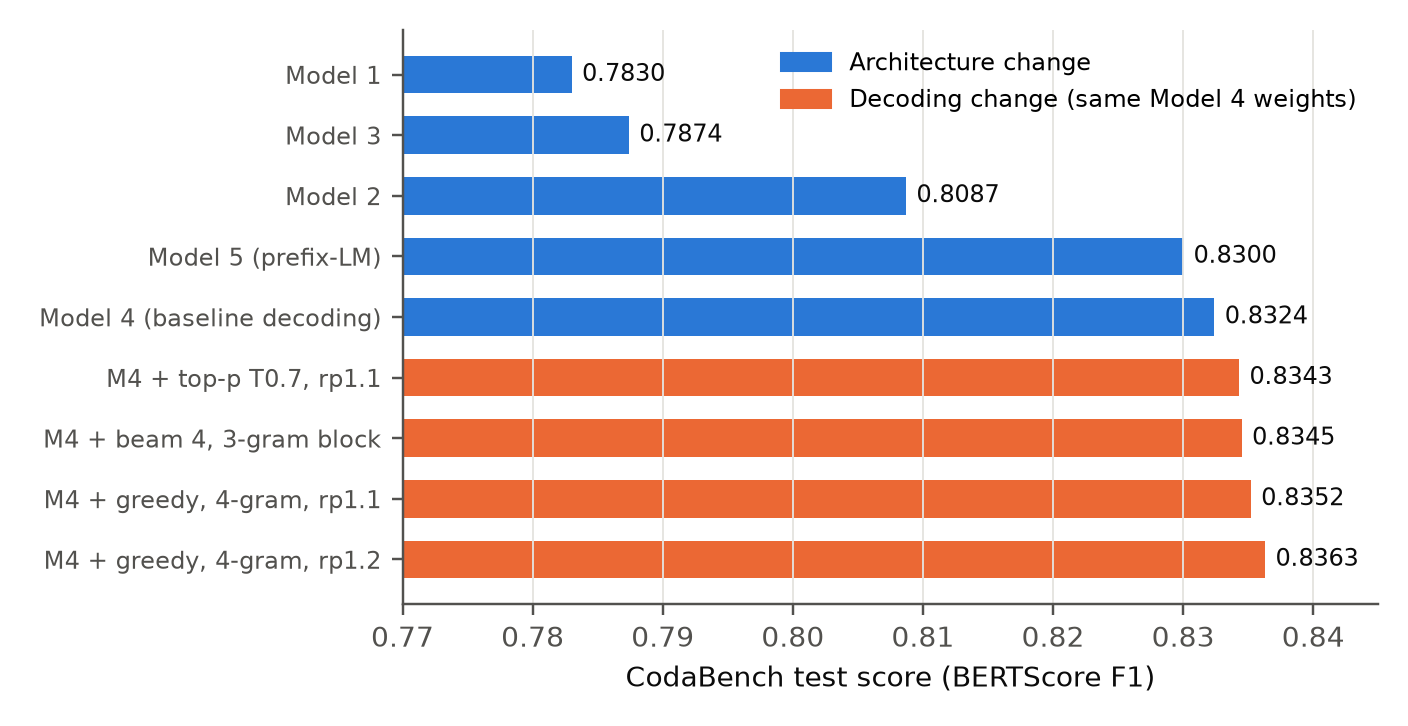
\includegraphics[width=\textwidth]{leaderboard.png}\caption{Codabench scores in the order the changes were made (blue: architectures, orange: decoding).}\end{subfigure}\hfill
\begin{subfigure}[t]{0.49\textwidth}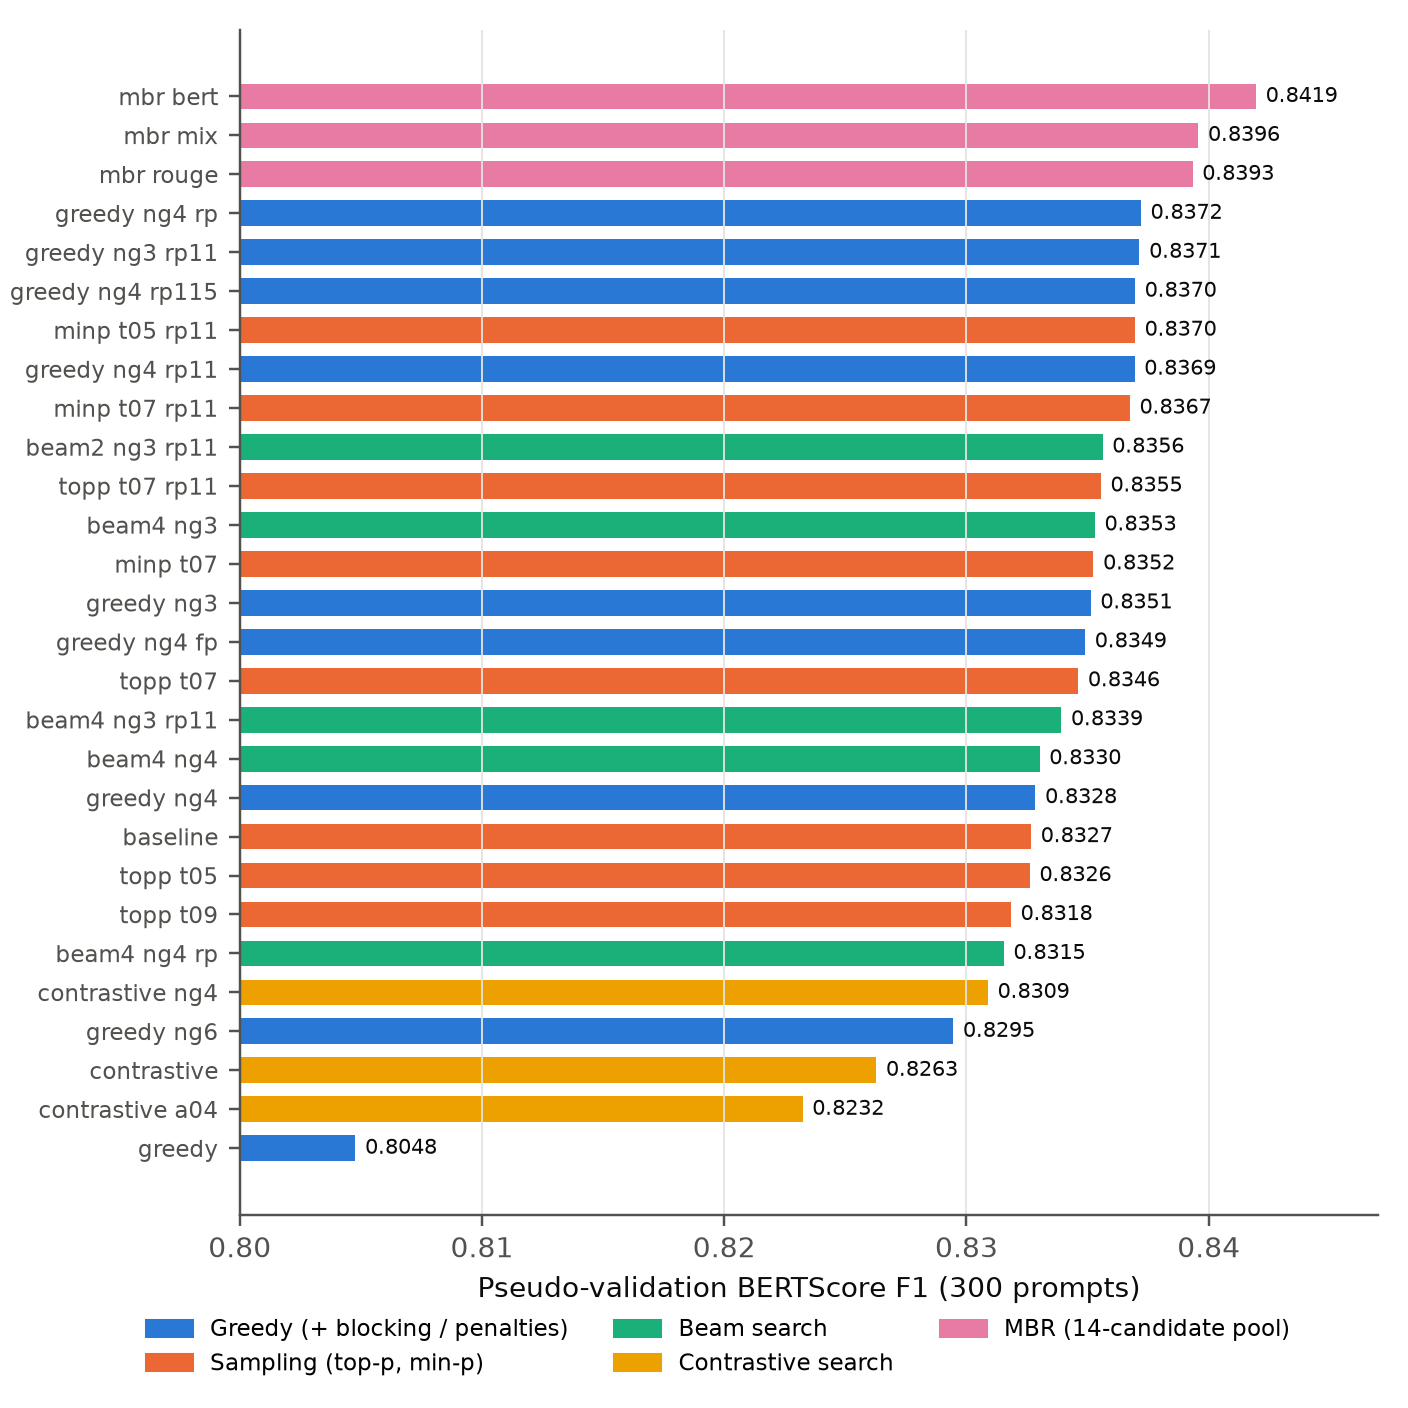
\includegraphics[width=\textwidth]{strategies.png}\caption{Pseudo-validation BERTScore of all 28 decoding settings on Model~4.}\end{subfigure}
\caption{Phase 1 progression and decoding study.}
\end{figure}

\section{Phase 2 details}\label{app:p2}
\begin{table}[H]
\centering\small
\caption{Phase 2 runs: strict macro-F1 / precision / recall on the 10 validation documents at the best epoch.}
\label{tab:p2runs}
\begin{adjustbox}{max width=\textwidth}
\begin{tabular}{llllrrccc r}
\toprule
Run & Model & Method & Output layer & Trained & Ep. & Val F1 & P & R & Codabench\\
\midrule
\run{m4\_lorma}          & M4 & LoRMA  & softmax & 1.13M  & 4 & 0.3202 & 0.305 & 0.368 & 0.3442\\
\run{m2\_lora}           & M2 & LoRA   & softmax & 1.04M  & 6 & 0.2899 & 0.269 & 0.325 & 0.3416\\
\run{m3\_full}           & M3 & full   & softmax & 68.4M  & 8 & 0.1906 & 0.204 & 0.187 & n/r\\
\run{m3\_bitfit}         & M3 & BitFit & softmax & 0.08M  & 7 & 0.1149 & 0.146 & 0.099 & n/r\\
\run{m4\_lorma\_vit}     & M4 & LoRMA  & constrained Viterbi & 1.13M & 6 & 0.4131 & 0.422 & 0.419 & n/r\\
\run{m4\_lorma\_crf}     & M4 & LoRMA  & CRF     & 1.13M  & 8 & 0.4502 & 0.531 & 0.415 & n/r\\
\run{m4\_full}           & M4 & full   & softmax & 101.4M & 7 & 0.3450 & 0.335 & 0.372 & n/r\\
\run{m4\_kd\_student}    & M4 (4 layers) & KD & softmax & 63.6M & 8 & 0.2841 & 0.259 & 0.322 & n/r\\
\run{m4\_small\_nokd}    & M4 (4 layers) & full (control) & softmax & 63.6M & 7 & 0.2695 & 0.241 & 0.314 & n/r\\
\run{m4\_lorma\_crf\_pre} & M4 & LoRMA & CRF + preamble 256 & 1.13M & 8 & 0.4561 & 0.555 & 0.419 & 0.4754$^*$\\
\run{m5\_lorma\_crf\_pre} & M5 & LoRMA & CRF + preamble 256 & 1.13M & 3 & \best{0.4797} & 0.517 & 0.470 & \best{0.5122}$^\dagger$\\
\bottomrule
\end{tabular}
\end{adjustbox}
\\[1pt]{\footnotesize Codabench of the run's own submission; $^*$+ propagate; $^\dagger$+ vote + propagate.
\run{m4\_lorma\_crf} + vote + propagate: validation 0.4813, Codabench 0.4715.}
\end{table}

\begin{table}[H]
\centering\small
\caption{Phase 2: gold $\to$ tags $\to$ spans round trip (strict macro-F1 ceiling) and validation strict macro-F1 of
the document-level rules.}
\label{tab:ceiling}
\begin{tabular}{lcc|lcccc}
\toprule
Trimming & train & val & Base & none & +vote & +prop. & +both\\
\midrule
none (raw token spans) & 0.605 & 0.650 & \run{m4\_lorma\_crf} & 0.4502 & 0.4591 & 0.4739 & 0.4813\\
basic (edge punctuation) & 0.947 & 0.932 & \run{m4\_lorma\_vit} & 0.4131 & 0.4153 & 0.4058 & 0.4079\\
smart (abbrev./bracket/possessive) & 0.979 & 0.973 & \run{m4\_full} & 0.3450 & 0.3475 & 0.3246 & 0.3275\\
\bottomrule
\end{tabular}
\end{table}

\begin{table}[H]
\centering\small
\caption{Phase 2 training documents: share whose first mention of a label lies within the first $P$ tokens, and share
of all mentions beyond token 1{,}024 (used to choose the preamble length).}
\label{tab:prefix}
\begin{tabular}{lcccccc}
\toprule
 & $P$=64 & 128 & 256 & 512 & 768 & $>$1024\\
\midrule
APP       & 90\% & 95\% & 98\% & 100\% & 100\% & 46\%\\
RESP      & 81\% & 90\% & 94\% & 97\%  & 98\%  & 55\%\\
JUDGE     & 62\% & 76\% & 77\% & 82\%  & 83\%  & 53\%\\
A.COUNSEL & 18\% & 24\% & 39\% & 43\%  & 51\%  & 53\%\\
R.COUNSEL & 11\% & 23\% & 36\% & 40\%  & 49\%  & 63\%\\
\bottomrule
\end{tabular}
\end{table}

\begin{figure}[H]
\centering
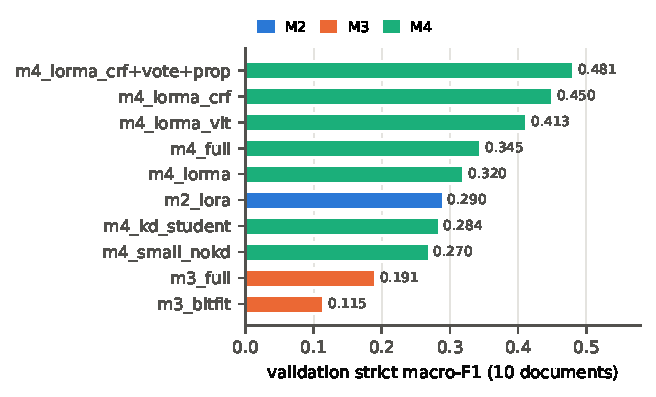
\includegraphics[width=0.55\textwidth]{p2_runs.pdf}
\caption{Phase 2 validation strict macro-F1 of the first two sessions' runs.}
\end{figure}

\section{Phase 3 details}\label{app:p3}
\begin{table}[H]
\centering\small
\caption{Phase 3 runs: dev macro-F1 and per-domain F1 (CL / IT); all runs read document windows.}
\label{tab:p3runs}
\begin{tabular}{llrcc}
\toprule
Run & Method / head & Trained & Dev & CL / IT\\
\midrule
\run{m2\_lora}   & LoRA / linear   & 1.03M & 0.415 & .361 / .416\\
\run{m2\_rslora} & rsLoRA / linear & 1.03M & 0.431 & .365 / .447\\
\run{m2\_lorma}  & LoRMA / linear  & 0.95M & 0.424 & .341 / .437\\
\run{m3}         & full / linear   & 68.3M & 0.205 & .182 / .209\\
\run{m4\_lora}   & LoRA / linear   & 1.10M & 0.435 & .368 / .413\\
\run{m4\_rslora} & rsLoRA / linear & 1.10M & 0.433 & .351 / .457\\
\run{m4\_lorma}  & LoRMA / linear  & 1.12M & 0.438 & .359 / .450\\
\run{m4\_full}   & full / linear   & 101M  & 0.437 & .343 / .443\\
\run{m5\_lora}   & LoRA / linear   & 1.10M & 0.441 & .354 / .418\\
\run{m5\_rslora} & rsLoRA / linear & 1.10M & 0.450 & .381 / .436\\
\run{m5\_lorma}  & LoRMA / linear  & 1.12M & 0.431 & .382 / .406\\
\run{m5\_full}   & full / linear   & 101M  & 0.442 & .374 / .447\\
\run{m5\_lora\_crf}   & LoRA / CRF   & 1.10M & \best{0.469} & .398 / .446\\
\run{m5\_rslora\_crf} & rsLoRA / CRF & 1.10M & 0.453 & .383 / .435\\
\run{m5\_lorma\_crf}  & LoRMA / CRF  & 1.12M & 0.427 & .368 / .425\\
\run{m5\_full\_crf}   & full / CRF   & 101M  & 0.455 & .378 / .461\\
\run{m5\_kd\_student} & KD 4 layers / linear & 63.6M & 0.347 & .265 / .390\\
\bottomrule
\end{tabular}
\end{table}

\begin{table}[H]
\centering\small
\caption{Phase 3 decoding strategies: dev macro-F1 (Codabench in brackets where submitted).}
\label{tab:p3pp}
\begin{tabular}{lcccc}
\toprule
Base & argmax / own CRF & prior & prior + Viterbi & + position prior\\
\midrule
\run{m2\_ens}  & 0.425 & 0.443 & 0.439 (0.495) & 0.422\\
\run{m3}       & 0.205 & 0.192 & 0.350 (0.334) & 0.353\\
\run{m4\_ens}  & 0.454 & 0.421 & 0.441 (0.525) & 0.453\\
\run{m5\_ens}  & 0.448 & 0.458 & 0.463 (0.562) & 0.465\\
\run{m5\_full\_crf} & 0.453 & 0.452 & 0.472 (0.543) & 0.496 (0.559)\\
\run{m5\_crf\_ens}  & 0.453 (0.504) & 0.457 & 0.471 (\best{0.571}) & 0.474 (0.556)\\
\bottomrule
\end{tabular}
\\[1pt]{\footnotesize Expected-F1 decoding of \run{m5\_crf\_ens} (coordinate ascent on HMM posteriors): dev 0.469,
Codabench 0.5657.}
\end{table}

\begin{figure}[H]
\centering
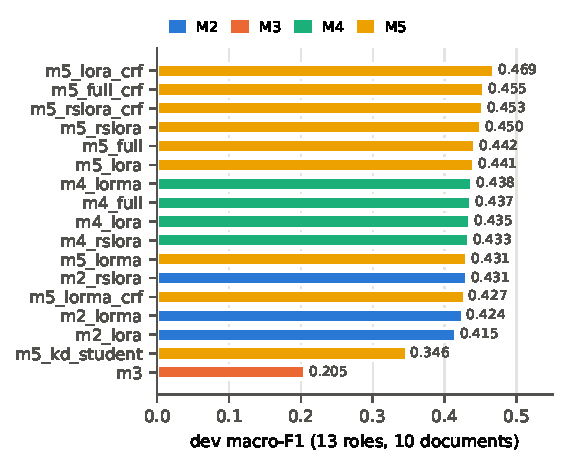
\includegraphics[width=0.55\textwidth]{p3_runs.pdf}
\caption{Phase 3 dev macro-F1 of all runs (argmax or the run's own CRF decoding).}
\end{figure}

\section{Phase 4 details}\label{app:p4}
\begin{table}[H]
\centering\small
\caption{Phase 4 runs: dev macro-F1 on the 994 development cases (argmax, reading the section the run was trained
on); Min.\ = training minutes on one T4.}
\label{tab:p4runs}
\begin{tabular}{lllrrrcr}
\toprule
Run & Method & Reads & Trained & Cases & Ep. & Dev F1 & Min.\\
\midrule
\run{m5\_rslora\_alldocs} & rslora & tail 1$\times$512 & 1.28M & 31.7k & 3 & 0.7087 & 186\\
\run{m5\_lora\_alldocs} & lora & tail 1$\times$512 & 1.28M & 31.7k & 3 & 0.6980 & 177\\
\run{m5\_full\_alldocs} & full & tail 1$\times$512 & 101.5M & 31.7k & 3 & 0.6874 & 201\\
\run{m2\_lorma} & lorma & tail 1$\times$512 & 1.14M & 10.0k & 3 & 0.6831 & 59\\
\run{m5\_rslora} & rslora & tail 1$\times$512 & 1.28M & 10.0k & 3 & 0.6615 & 65\\
\run{m2\_lora} & lora & tail 1$\times$512 & 1.22M & 10.0k & 2 & 0.6609 & 58\\
\run{m5\_lorma\_hier4} & lorma & tail 4$\times$512 & 1.30M & 10.0k & 3 & 0.6566 & 192\\
\run{m5\_full} & full & tail 1$\times$512 & 101.5M & 10.0k & 1 & 0.6528 & 69\\
\run{m5\_lorma\_alldocs} & lorma & tail 1$\times$512 & 1.30M & 31.7k & 3 & 0.6519 & 175\\
\run{m5\_kd\_student} & kd & tail 1$\times$512 & 63.8M & 10.0k & 2 & 0.6503 & 26\\
\run{m4\_rslora} & rslora & tail 1$\times$512 & 1.28M & 10.0k & 1 & 0.6415 & 65\\
\run{m5\_lora} & lora & tail 1$\times$512 & 1.28M & 10.0k & 3 & 0.6398 & 65\\
\run{m4\_full} & full & tail 1$\times$512 & 101.5M & 10.0k & 2 & 0.6389 & 69\\
\run{m2\_rslora} & rslora & tail 1$\times$512 & 1.22M & 10.0k & 3 & 0.6384 & 59\\
\run{m4\_lorma} & lorma & tail 1$\times$512 & 1.30M & 10.0k & 1 & 0.6318 & 64\\
\run{m5\_lorma} & lorma & tail 1$\times$512 & 1.30M & 10.0k & 3 & 0.6233 & 64\\
\run{m4\_lora} & lora & tail 1$\times$512 & 1.28M & 10.0k & 1 & 0.6224 & 65\\
\run{m3} & full & tail 1$\times$512 & 68.8M & 10.0k & 3 & 0.5901 & 11\\
\run{m5\_lorma\_head} & lorma & head 1$\times$512 & 1.30M & 10.0k & 3 & 0.5602 & 58\\
\bottomrule
\end{tabular}

\end{table}

\begin{table}[H]
\centering\small
\caption{Phase 4 submissions: dev, 2-fold CV and Codabench macro-F1.}
\begin{tabular}{lccc}
\toprule
Submission & Dev & CV & Codabench\\
\midrule
\run{m5\_rslora}, both readings, dev threshold & 0.7003 & 0.6924 & 0.6941\\
\run{m2\_lorma}, both readings, training-prior threshold & 0.7188 & (fixed rule) & 0.6889\\
\run{m5\_rslora\_alldocs}, last $8\times512$, dev threshold & 0.7665 & 0.7537 & 0.7374\\
\run{m5\_alldocs\_ens}, last $8\times512$, dev threshold & 0.7612 & 0.7521 & \best{0.7609}\\
\run{m5\_alldocs\_ens}, both readings, dev threshold & 0.7594 & 0.7484 & 0.7523\\
\bottomrule
\end{tabular}
\end{table}

\begin{figure}[H]
\centering
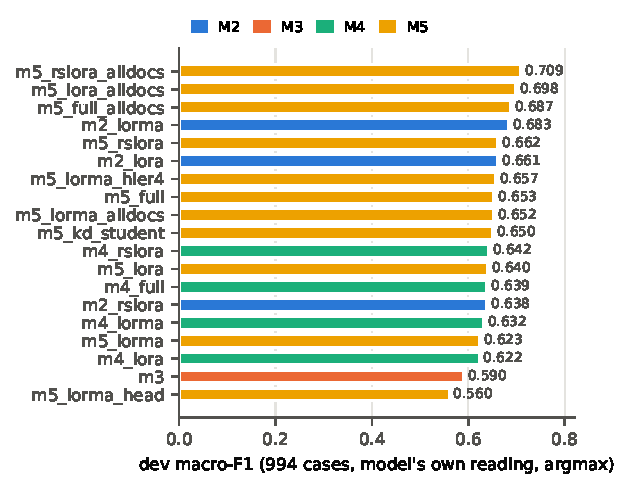
\includegraphics[width=0.55\textwidth]{p4_runs.pdf}
\caption{Phase 4 dev macro-F1 of every run.}
\end{figure}

\section{Phase 5 details}\label{app:p5}
\begin{table}[H]
\centering\small
\caption{Phase 5 runs: full-dev macro-F1 and micro-F1 with one global threshold (Thr.).}
\label{tab:p5runs}
\begin{tabular}{lllrrrccc}
\toprule
Run & Method & Reads & Trained & Docs & Ep. & Dev F1 & Micro & Thr.\\
\midrule
\run{m4\_full} & full & head 4$\times$512 & 101.6M & 15k & 3 & 0.3535 & 0.481 & 0.18\\
\run{m5\_full} & full & head 4$\times$512 & 101.6M & 15k & 3 & 0.3531 & 0.480 & 0.18\\
\run{m5\_lorma\_head1\_alldocs} & lorma & head 1$\times$512 & 1.38M & 42k & 3 & 0.3490 & 0.470 & 0.16\\
\run{m5\_kd\_student} & kd & head 4$\times$512 & 63.8M & 15k & 3 & 0.3460 & 0.466 & 0.14\\
\run{m4\_lorma} & lorma & head 4$\times$512 & 1.38M & 15k & 3 & 0.3414 & 0.468 & 0.16\\
\run{m5\_partial} & partial & head 4$\times$512 & 31.7M & 15k & 3 & 0.3364 & 0.466 & 0.16\\
\run{m5\_lorma\_sqrtpw} & lorma & head 4$\times$512 & 1.38M & 15k & 3 & 0.3355 & 0.439 & 0.52\\
\run{m5\_lorma} & lorma & head 4$\times$512 & 1.38M & 15k & 3 & 0.3292 & 0.459 & 0.16\\
\run{m2\_lorma} & lorma & head 4$\times$512 & 1.22M & 15k & 3 & 0.3278 & 0.448 & 0.14\\
\run{m3} & full & head 4$\times$512 & 69.0M & 15k & 3 & 0.2105 & 0.346 & 0.08\\
\bottomrule
\end{tabular}

\end{table}

\begin{figure}[H]
\centering
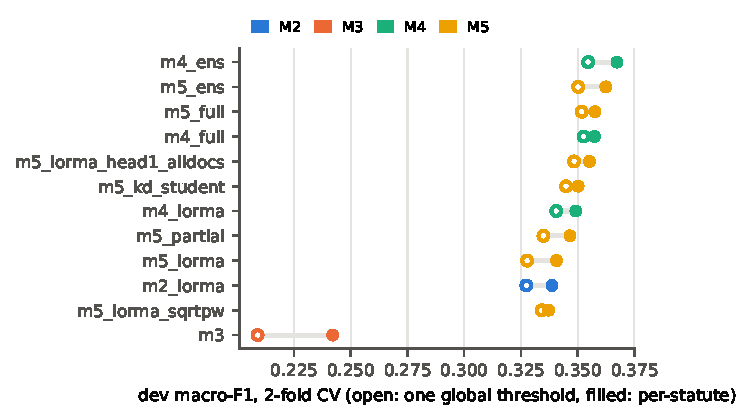
\includegraphics[width=0.6\textwidth]{p5_thresholds.pdf}
\caption{Phase 5 dev macro-F1 (2-fold CV) with one global threshold (open) and per-statute thresholds (filled).}
\end{figure}

\section{Phase 6 details}\label{app:p6}
\begin{table}[H]
\centering\small
\caption{Phase 6 runs: held-out loss and the 100 generated held-out summaries (BERTScore F1, ROUGE-1/L, mean length in
words; references average 852 words).}
\label{tab:p6runs}
\begin{tabular}{llrrcccccr}
\toprule
Run & Method & Trained & Ep. & Val loss & BERTScore & R-1 & R-L & Words & Min.\\
\midrule
\run{m4\_lora} & lora & 1.09M & 2 & 2.570 & 0.8378 & 0.447 & 0.236 & 535 & 122\\
\run{m2\_houlsby} & houlsby & 2.01M & 2 & 2.519 & 0.8377 & 0.459 & 0.238 & 664 & 113\\
\run{m5\_lorma} & lorma & 1.11M & 2 & 2.685 & 0.8361 & 0.442 & 0.237 & 630 & 121\\
\run{m5\_kd\_student} & kd & 63.6M & 2 & 3.798 & 0.8232 & 0.407 & 0.224 & 566 & 103\\
\run{m3\_full} & full & 91.7M & 0.94 & 4.444 & 0.8033 & 0.319 & 0.174 & 747 & 81\\
\bottomrule
\end{tabular}

\end{table}

\begin{table}[H]
\centering\small
\caption{Phase 6 decoding variants and ensembles on the held-out set, and Codabench.}
\begin{tabular}{lccc}
\toprule
System & Held-out BERTScore & ROUGE-1 & Codabench\\
\midrule
\run{m4\_lora}, repetition penalty 1.15 & 0.8423 & --- & \best{0.8381}\\
\run{m4\_lora}, 3-gram block & 0.8414 & --- & 0.8380\\
MBR consensus over all runs & 0.8398 & 0.476 & n/r\\
MBR over \run{m4\_lora} variants & 0.8376 & --- & n/r\\
MBR over \run{m2\_houlsby} variants & 0.8371 & --- & n/r\\
\bottomrule
\end{tabular}
\end{table}

\begin{figure}[H]
\centering
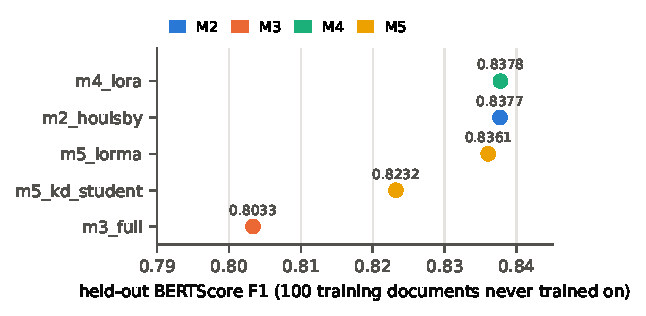
\includegraphics[width=0.55\textwidth]{p6_bertscore.pdf}
\caption{Phase 6 held-out BERTScore F1 of every run (greedy, no-repeat 4-grams).}
\end{figure}

\section{Phase 7 details}\label{app:p7}
\begin{table}[H]
\centering\small
\caption{Phase 7 runs: dev Micro-F1@7 of the untrained Phase 1 encoder (0-shot) and at the best epoch, recall in the
top 100; raw cosine ranking with the date and self rules. The two Model~2 runs did not run (dataset not attached).}
\label{tab:p7runs}
\begin{tabular}{lllrrcccr}
\toprule
Run & Method & Layers & Trained & Ep. & 0-shot & Dev F1@7 & R@100 & Min.\\
\midrule
\run{m5\_full} & full & 10/10 & 101.3M & 5 & 0.2424 & 0.3146 & 0.680 & 35\\
\run{m4\_full} & full & 10/10 & 101.3M & 6 & 0.2457 & 0.3102 & 0.700 & 34\\
\run{m5\_lorma} & lorma & 10/10 & 1.11M & 6 & 0.2424 & 0.3091 & 0.692 & 37\\
\run{m5\_kd\_student} & kd & 4/10 & 63.6M & 5 & 0.2379 & 0.2913 & 0.690 & 14\\
\run{m3\_full} & full & 2/2 & 68.3M & 4 & 0.1467 & 0.2724 & 0.660 & 16\\
\run{m4\_ia3} & ia3 & 10/10 & 0.03M & 4 & 0.2457 & 0.2690 & 0.668 & 33\\
\bottomrule
\end{tabular}

\end{table}

\begin{table}[H]
\centering\small
\caption{Phase 7 post-processing: raw ranking, dev-selected setting (Dev), its 2-fold CV estimate, the same without the
query penalty ($^-$), and Codabench (-- = not submitted). M5 LoRMA reading 4 chunks: \run{head4} 0.3302, \run{spread4}
0.3413 raw.}
\label{tab:p7pp}
\begin{tabular}{lccccccc}
\toprule
Base & Raw & Dev & CV & Dev$^-$ & CV$^-$ & LB & LB$^-$\\
\midrule
\run{bm25} & 0.1857 & 0.4325 & 0.4264 & 0.4269 & 0.4249 & 0.4306 & 0.4318\\
\run{m3\_full} & 0.2724 & 0.4325 & 0.4263 & 0.4258 & 0.4200 & -- & --\\
\run{m4\_full} & 0.3102 & 0.4336 & 0.4280 & 0.4280 & 0.4228 & 0.4253 & --\\
\run{m4\_ia3} & 0.2690 & 0.4336 & 0.4257 & 0.4280 & 0.4236 & -- & --\\
\run{m5\_full} & 0.3146 & 0.4369 & 0.4311 & 0.4280 & 0.4240 & 0.4288 & --\\
\run{m5\_lorma} & 0.3091 & 0.4369 & 0.4308 & 0.4258 & 0.4202 & -- & --\\
\run{m5\_lorma\_\_head1} & 0.2779 & 0.4369 & 0.4331 & 0.4269 & 0.4223 & 0.4259 & --\\
\run{m5\_lorma\_\_spread4} & 0.3413 & 0.4380 & 0.4317 & 0.4269 & 0.4200 & 0.4300 & --\\
\run{m5\_kd\_student} & 0.2913 & 0.4314 & 0.4251 & 0.4269 & 0.4226 & -- & --\\
\run{all\_ens} & 0.3191 & 0.4347 & 0.4284 & 0.4291 & 0.4245 & 0.4300 & 0.4318\\
\bottomrule
\end{tabular}

\end{table}

\begin{figure}[H]
\centering
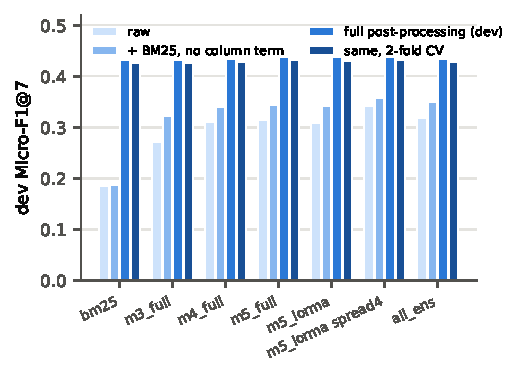
\includegraphics[width=0.55\textwidth]{p7_postprocess.pdf}
\caption{Phase 7 post-processing steps on dev.}
\end{figure}

\section{Implementation details}\label{app:impl}
\textbf{Parallel CRF partition function (Phase~2).} The linear-chain CRF scores a tag sequence as
$s(y)=\mathit{start}[y_0]+\sum_t \mathit{em}[t,y_t]+\sum_{t\ge1}\mathit{trans}[y_{t-1},y_t]+\mathit{end}[y_{n-1}]$ and is
trained on $\log Z-s(y_\text{gold})$ per tagged token, with invalid BIO transitions fixed at $-10^4$. The sequential
forward recursion for $\log Z$ took 3.8\,s per batch of four 1{,}024-token windows. Writing each step as a $25\times25$
matrix $M_t[i,j]=\mathit{trans}[i,j]+\mathit{em}[t,j]$ in the log semiring (where ``multiplication'' is log-sum-exp of
sums) and multiplying neighbours pairwise needs $\log_2 1024=10$ parallel rounds: 0.036\,s per batch, with results equal
to the sequential recursion and to brute-force enumeration on short sequences. The CRF adds 675 parameters.

\textbf{Preamble context (Phase~2).} With \texttt{preamble\_tokens}$=P$, every window not starting at the document start
receives the document's first $P$ tokens in front of its content (content shrinks to $1024-P$); these positions carry no
loss, no distillation signal and no predictions. $P=256$ covers the first appellant/respondent mention in 98\%/94\% of
training documents (Table~\ref{tab:prefix}); $P=512$ would remove the window overlap.

\textbf{Decoding from training statistics (Phase~3).} With per-sentence posteriors $p(y\mid x_t)$, the prior strategy
decodes $\arg\max_y \log p(y\mid x_t)-\log\pi(y)$ with the training role frequencies $\pi$; prior + Viterbi finds the
role sequence maximising $\sum_t[\log p(y_t\mid x_t)-\log\pi(y_t)]+\sum_t\log A(y_{t-1},y_t)$ with training transition
probabilities $A$; the position prior adds $\log p(y\mid b_t)-\log\pi(y)$ for 10 relative-position bins $b_t$. CRF runs
are first converted to per-sentence posteriors by forward--backward with their learned transitions.

\textbf{Gradient caching (Phase~7).} A batch of 16 queries with one positive and one hard negative each holds about 48
cases of 1{,}024 tokens. I (i) encode all cases without gradients, (ii) compute the InfoNCE loss and its gradient with
respect to the embedding matrix, and (iii) re-encode each sub-batch of $\le$4{,}096 tokens with gradients and
back-propagate the cached embedding gradient into it. Parameter gradients matched direct back-propagation to a relative
$10^{-6}$, and a single batch could be over-fitted (loss 2.65 $\to$ 0.0016). The KD student matches the teacher's
in-batch similarity distributions (teacher embeddings of the training cases are pre-computed once).

\section{Code and reproducibility}\label{app:code}
The repository \url{https://github.com/D3bug1t/LLM-Pretraining-PostTraining-Extrinsic-Instrinsic-Evals} (and the
\texttt{code/} folder of the submitted archive) contains the phase notebooks, post-processing scripts and official
evaluation scripts, with a README per phase. The Phase~2--7 figures and appendix tables are generated from saved results by \texttt{make\_figures.py}
and \texttt{data\_stats.py}. The separate course-required LLM analysis is
\texttt{llm\_based\_results\_and\_data\_analysis.pdf}.

\end{document}
